\documentclass{article}
\usepackage[T1]{fontenc}
\usepackage{times}
\usepackage{iclr2027_conference,times}
\usepackage{amsmath,amssymb,amsthm}
\usepackage{booktabs}
\usepackage{graphicx}
\usepackage{url}
\usepackage{hyperref}

\newtheorem{theorem}{Theorem}
\newtheorem{proposition}{Proposition}
\newtheorem{corollary}{Corollary}
\newtheorem{assumption}{Assumption}

% Numbers quoted in running text, generated by analysis/story_tables.py from
% committed raw outputs.
% generated by analysis/story_tables.py
\newcommand{\ContestBpbacktrack}{0}
\newcommand{\ContestBpcavity}{0}
\newcommand{\ContestBptrw}{0}
\newcommand{\ContestCovint}{85}
\newcommand{\ContestEcexact}{100}
\newcommand{\ContestInvcovint}{80}
\newcommand{\ContestMeanpool}{80}
\newcommand{\ContestNaivesum}{0}
\newcommand{\ContestSeeds}{20}
\newcommand{\ReaderCanonExactRecall}{0.5083}
\newcommand{\ReaderCanonExactTokens}{318.9}
\newcommand{\ReaderCanonOverlapRecall}{0.4500}
\newcommand{\ReaderCanonOverlapTokens}{473.9}
\newcommand{\ReaderExactRatio}{11.6}
\newcommand{\ReaderLedgerExactRecall}{0.5083}
\newcommand{\ReaderLedgerExactTokens}{318.9}
\newcommand{\ReaderLedgerOverlapRecall}{0.4667}
\newcommand{\ReaderLedgerOverlapTokens}{341.9}
\newcommand{\ReaderOverlapRatio}{6.4}
\newcommand{\ReaderPlainExactRecall}{0.4917}
\newcommand{\ReaderPlainExactTokens}{3710.0}
\newcommand{\ReaderPlainOverlapRecall}{0.4333}
\newcommand{\ReaderPlainOverlapTokens}{2175.2}
\newcommand{\ReaderRecords}{120}
\newcommand{\SyndCanonBoiler}{+0.1333}
\newcommand{\SyndCanonBoilerCI}{[+0.0833, +0.1833]}
\newcommand{\SyndCanonBoilerMisled}{-0.1400}
\newcommand{\SyndCanonBoilerMisledCI}{[-0.1800, -0.1000]}
\newcommand{\SyndCanonPlain}{+0.0000}
\newcommand{\SyndCanonPlainCI}{[+0.0000, +0.0000]}
\newcommand{\SyndDrop}{-0.1167}
\newcommand{\SyndDropCI}{[-0.1600, -0.0733]}
\newcommand{\SyndFirstPlainGold}{+0.0233}
\newcommand{\SyndFirstPlainGoldCI}{[-0.0200, +0.0667]}
\newcommand{\SyndFirstPlainMisled}{-0.0267}
\newcommand{\SyndFirstPlainMisledCI}{[-0.0500, -0.0033]}
\newcommand{\SyndGain}{+0.1167}
\newcommand{\SyndGainCI}{[+0.0733, +0.1600]}
\newcommand{\SyndHeld}{5}
\newcommand{\SyndLedgerTokens}{464.5}
\newcommand{\SyndMinhashFirst}{+0.3300}
\newcommand{\SyndMinhashFirstBoiler}{+0.2000}
\newcommand{\SyndMinhashFirstBoilerCI}{[+0.1567, +0.2467]}
\newcommand{\SyndMinhashFirstCI}{[+0.2767, +0.3833]}
\newcommand{\SyndMinhashLast}{-0.0367}
\newcommand{\SyndMinhashLastCI}{[-0.0667, -0.0067]}
\newcommand{\SyndMinhashTrueKept}{0.4767}
\newcommand{\SyndMinhashTrueLost}{52}
\newcommand{\SyndMisledOne}{0.0100}
\newcommand{\SyndMisledRise}{+0.1267}
\newcommand{\SyndMisledRiseCI}{[+0.0900, +0.1667]}
\newcommand{\SyndMisledSixteen}{0.1367}
\newcommand{\SyndPlainOne}{0.5133}
\newcommand{\SyndPlainSixteen}{0.3967}
\newcommand{\SyndPlainTokens}{2362.1}
\newcommand{\SyndPredictions}{5}
\newcommand{\SyndSimBoiler}{+0.0633}
\newcommand{\SyndSimBoilerCI}{[+0.0200, +0.1067]}
\newcommand{\SyndTokenRatio}{5.1}

% generated by analysis/learned_memory_table.py
\newcommand{\FragmentsArmReady}{1}
\newcommand{\LmDedupOverlapFour}{0.0588}
\newcommand{\LmExactAccGain}{+0.0318}
\newcommand{\LmExactAccGainCI}{[+0.0168, +0.0468]}
\newcommand{\LmExactMrrGain}{+0.0411}
\newcommand{\LmExactMrrGainCI}{[+0.0294, +0.0529]}
\newcommand{\LmExactNllGain}{-0.8799}
\newcommand{\LmExactNllGainCI}{[-1.1124, -0.6474]}
\newcommand{\LmFragAccGain}{+0.0064}
\newcommand{\LmFragAccGainCI}{[-0.0059, +0.0187]}
\newcommand{\LmFragArrivals}{32}
\newcommand{\LmFragBestDetector}{MinHash}
\newcommand{\LmFragDetGain}{-0.0019}
\newcommand{\LmFragDetGainCI}{[-0.0102, +0.0064]}
\newcommand{\LmFragLedgerCredit}{1.000}
\newcommand{\LmFragLedgerReach}{7.5}
\newcommand{\LmFragMrrGain}{+0.0114}
\newcommand{\LmFragMrrGainCI}{[-0.0007, +0.0235]}
\newcommand{\LmFragNllGain}{-0.1987}
\newcommand{\LmFragNllGainCI}{[-0.3597, -0.0376]}
\newcommand{\LmFragPlainCredit}{16.000}
\newcommand{\LmLedgerClean}{0.1141}
\newcommand{\LmLedgerExactSixteen}{0.1141}
\newcommand{\LmLedgerOverlapFour}{0.0791}
\newcommand{\LmLedgerOverlapSixteen}{0.0791}
\newcommand{\LmOverlapAccGain}{-0.0040}
\newcommand{\LmOverlapAccGainCI}{[-0.0135, +0.0055]}
\newcommand{\LmPlainExactSixteen}{0.0823}
\newcommand{\LmPlainOverlapFour}{0.0919}
\newcommand{\LmPlainOverlapSixteen}{0.0831}
\newcommand{\LmRechunkAccGain}{+0.0326}
\newcommand{\LmRechunkAccGainCI}{[+0.0147, +0.0505]}
\newcommand{\LmRechunkBestDetector}{embedding detection}
\newcommand{\LmRechunkDetGain}{+0.0307}
\newcommand{\LmRechunkDetGainCI}{[+0.0226, +0.0388]}
\newcommand{\LmRechunkLedgerClean}{0.1141}
\newcommand{\LmRechunkLedgerSixteen}{0.1141}
\newcommand{\LmRechunkMrrGain}{+0.0486}
\newcommand{\LmRechunkMrrGainCI}{[+0.0344, +0.0628]}
\newcommand{\LmRechunkNllGain}{-1.1882}
\newcommand{\LmRechunkNllGainCI}{[-1.4350, -0.9414]}
\newcommand{\LmRechunkPlainSixteen}{0.0815}
\newcommand{\RechunkArmReady}{1}

% generated by analysis/directional_analysis.py
\newcommand{\DirReBestFloor}{0.2747}
\newcommand{\DirReBestMinPooled}{0.7404}
\newcommand{\DirReBestMinStrat}{0.7132}
\newcommand{\DirReBestVsMean}{+0.0202}
\newcommand{\DirReBestVsMeanCI}{[+0.0023, +0.0379]}
\newcommand{\DirReDPooled}{0.6989}
\newcommand{\DirReDStrat}{0.6563}
\newcommand{\DirReDupLinD}{0.6989}
\newcommand{\DirReDupNoneD}{0.6874}
\newcommand{\DirReDupNoneS}{0.6508}
\newcommand{\DirReDvsBestMin}{-0.0569}
\newcommand{\DirReDvsBestMinCI}{[-0.0747, -0.0400]}
\newcommand{\DirReDvsSumCos}{+0.1892}
\newcommand{\DirReDvsSumCosCI}{[+0.1592, +0.2169]}
\newcommand{\DirReHopsPooled}{0.7018}
\newcommand{\DirReHopsStrat}{0.5000}
\newcommand{\DirReLinEffD}{+0.0116}
\newcommand{\DirReLinEffDCI}{[+0.0018, +0.0210]}
\newcommand{\DirReLinEffS}{-0.0490}
\newcommand{\DirReLinEffSCI}{[-0.0582, -0.0397]}
\newcommand{\DirReMaxCosStrat}{0.5467}
\newcommand{\DirReMeanBestStrat}{0.6930}
\newcommand{\DirReN}{2{,}417}
\newcommand{\DirReROne}{+0.1535}
\newcommand{\DirReROneCI}{[+0.1312, +0.1755]}
\newcommand{\DirReROnePooled}{+0.0971}
\newcommand{\DirReROnePooledCI}{[+0.0784, +0.1156]}
\newcommand{\DirReRTwo}{+0.0481}
\newcommand{\DirReRTwoCI}{[+0.0294, +0.0673]}
\newcommand{\DirReSPooled}{0.6019}
\newcommand{\DirReSStrat}{0.5028}
\newcommand{\DirReSufficient}{0.403}
\newcommand{\DirReSumCosPooled}{0.5006}
\newcommand{\DirReSumCosStrat}{0.4671}
\newcommand{\DirSynGapFour}{+0.2282}
\newcommand{\DirSynGapFourCI}{[+0.1173, +0.3392]}
\newcommand{\DirSynGapOne}{+0.1103}
\newcommand{\DirSynGapTwo}{+0.1426}
\newcommand{\DirSynSOne}{+0.1103}
\newcommand{\DirSynSOneCI}{[-0.1765, +0.3971]}
\newcommand{\DirSynSOneFixed}{+0.2604}
\newcommand{\DirSynSOneFixedCI}{[-0.0978, +0.6186]}
\newcommand{\DirSynSTwo}{+21.8666}
\newcommand{\DirSynSTwoCI}{[+4.9638, +38.7694]}

% Generated by analysis/final_paper_macros.py from committed reports.
% Do not edit by hand; regenerate instead.
\newcommand{\MsqFitRecords}{17,185}
\newcommand{\MsqValRecords}{926}
\newcommand{\MsqParams}{493,824}
\newcommand{\MsqSeeds}{5}
\newcommand{\MsqNTwo}{1,252}
\newcommand{\MsqCandTwo}{555}
\newcommand{\MsqFullTwo}{0.1141}
\newcommand{\MsqFilterTwo}{0.0145}
\newcommand{\MsqDiffTwo}{+0.0995}
\newcommand{\MsqCITwo}{[0.0894, 0.1096]}
\newcommand{\MsqFullMrrTwo}{0.1987}
\newcommand{\MsqFullCosTwo}{0.4103}
\newcommand{\MsqFilterOnlyMrrTwo}{0.0407}
\newcommand{\MsqFilterOnlyCosTwo}{0.3738}
\newcommand{\MsqNoProvenanceMrrTwo}{0.1987}
\newcommand{\MsqNoProvenanceCosTwo}{0.4103}
\newcommand{\MsqPlainMrrTwo}{0.1987}
\newcommand{\MsqPlainCosTwo}{0.4103}
\newcommand{\MsqNThree}{568}
\newcommand{\MsqCandThree}{134}
\newcommand{\MsqFullThree}{0.2380}
\newcommand{\MsqFilterThree}{0.0229}
\newcommand{\MsqDiffThree}{+0.2151}
\newcommand{\MsqCIThree}{[0.1460, 0.2843]}
\newcommand{\MsqFullMrrThree}{0.3805}
\newcommand{\MsqFullCosThree}{0.3846}
\newcommand{\MsqFilterOnlyMrrThree}{0.0763}
\newcommand{\MsqFilterOnlyCosThree}{0.3769}
\newcommand{\MsqNoProvenanceMrrThree}{0.3805}
\newcommand{\MsqNoProvenanceCosThree}{0.3846}
\newcommand{\MsqPlainMrrThree}{0.3805}
\newcommand{\MsqPlainCosThree}{0.3846}
\newcommand{\MsqNFour}{246}
\newcommand{\MsqCandFour}{61}
\newcommand{\MsqFullFour}{0.2772}
\newcommand{\MsqFilterFour}{0.0154}
\newcommand{\MsqDiffFour}{+0.2618}
\newcommand{\MsqCIFour}{[0.2192, 0.3044]}
\newcommand{\MsqFullMrrFour}{0.3976}
\newcommand{\MsqFullCosFour}{0.3790}
\newcommand{\MsqFilterOnlyMrrFour}{0.0870}
\newcommand{\MsqFilterOnlyCosFour}{0.3832}
\newcommand{\MsqNoProvenanceMrrFour}{0.3976}
\newcommand{\MsqNoProvenanceCosFour}{0.3790}
\newcommand{\MsqPlainMrrFour}{0.3976}
\newcommand{\MsqPlainCosFour}{0.3790}
\newcommand{\MsqFullRedelivery}{1.0}
\newcommand{\MsqFullCycle}{1.0}
\newcommand{\MsqFilterOnlyRedelivery}{1.0}
\newcommand{\MsqFilterOnlyCycle}{1.0}
\newcommand{\MsqNoProvenanceRedelivery}{16.0}
\newcommand{\MsqNoProvenanceCycle}{16.0}
\newcommand{\MsqPlainRedelivery}{16.0}
\newcommand{\MsqPlainCycle}{16.0}
\newcommand{\MsqMaxDrift}{0.0}
\newcommand{\MsqContentPathMaxDelta}{0}
\newcommand{\MsqLicense}{CC BY 4.0}
\newcommand{\MsqTrainRecords}{19,938}
\newcommand{\MsqTrainLinear}{18,759}
\newcommand{\MsqTrainLinearPct}{94.1}
\newcommand{\MsqDevRecords}{2,417}
\newcommand{\MsqDevLinear}{2,066}
\newcommand{\SybPopulation}{200}
\newcommand{\SybEligible}{60}
\newcommand{\SybEligibilityPct}{30}
\newcommand{\SybThreshold}{0.88936}
\newcommand{\SybSurfaceThreshold}{0.87}
\newcommand{\SybRecall}{0.9354}
\newcommand{\SybFalseLinkPct}{0.50}
\newcommand{\SybPositivePairs}{15,030}
\newcommand{\SybNegativePairs}{9,233}
\newcommand{\SybUrlOneRatio}{1.000}
\newcommand{\SybUrlOneCI}{[1.000, 1.000]}
\newcommand{\SybUrlOneNLL}{1.1212}
\newcommand{\SybUrlOneFlip}{0.0000}
\newcommand{\SybUrlTwoRatio}{2.060}
\newcommand{\SybUrlTwoCI}{[1.995, 2.126]}
\newcommand{\SybUrlTwoNLL}{1.1056}
\newcommand{\SybUrlTwoFlip}{0.0467}
\newcommand{\SybUrlFourRatio}{4.131}
\newcommand{\SybUrlFourCI}{[4.030, 4.233]}
\newcommand{\SybUrlFourNLL}{1.1496}
\newcommand{\SybUrlFourFlip}{0.0433}
\newcommand{\SybUrlEightRatio}{4.567}
\newcommand{\SybUrlEightCI}{[4.328, 4.807]}
\newcommand{\SybUrlEightNLL}{1.1394}
\newcommand{\SybUrlEightFlip}{0.0600}
\newcommand{\SybCanonicalOneRatio}{1.000}
\newcommand{\SybCanonicalOneCI}{[1.000, 1.000]}
\newcommand{\SybCanonicalOneNLL}{1.1212}
\newcommand{\SybCanonicalOneFlip}{0.0000}
\newcommand{\SybCanonicalTwoRatio}{2.060}
\newcommand{\SybCanonicalTwoCI}{[1.995, 2.126]}
\newcommand{\SybCanonicalTwoNLL}{1.1056}
\newcommand{\SybCanonicalTwoFlip}{0.0467}
\newcommand{\SybCanonicalFourRatio}{4.131}
\newcommand{\SybCanonicalFourCI}{[4.030, 4.233]}
\newcommand{\SybCanonicalFourNLL}{1.1496}
\newcommand{\SybCanonicalFourFlip}{0.0433}
\newcommand{\SybCanonicalEightRatio}{4.567}
\newcommand{\SybCanonicalEightCI}{[4.328, 4.807]}
\newcommand{\SybCanonicalEightNLL}{1.1394}
\newcommand{\SybCanonicalEightFlip}{0.0600}
\newcommand{\SybSurfaceOneRatio}{1.000}
\newcommand{\SybSurfaceOneCI}{[1.000, 1.000]}
\newcommand{\SybSurfaceOneNLL}{1.1212}
\newcommand{\SybSurfaceOneFlip}{0.0000}
\newcommand{\SybSurfaceTwoRatio}{2.016}
\newcommand{\SybSurfaceTwoCI}{[1.945, 2.088]}
\newcommand{\SybSurfaceTwoNLL}{1.1046}
\newcommand{\SybSurfaceTwoFlip}{0.0467}
\newcommand{\SybSurfaceFourRatio}{3.363}
\newcommand{\SybSurfaceFourCI}{[3.230, 3.497]}
\newcommand{\SybSurfaceFourNLL}{1.1302}
\newcommand{\SybSurfaceFourFlip}{0.0433}
\newcommand{\SybSurfaceEightRatio}{3.724}
\newcommand{\SybSurfaceEightCI}{[3.514, 3.933]}
\newcommand{\SybSurfaceEightNLL}{1.1198}
\newcommand{\SybSurfaceEightFlip}{0.0600}
\newcommand{\SybSemanticOneRatio}{1.000}
\newcommand{\SybSemanticOneCI}{[1.000, 1.000]}
\newcommand{\SybSemanticOneNLL}{1.1212}
\newcommand{\SybSemanticOneFlip}{0.0000}
\newcommand{\SybSemanticTwoRatio}{1.676}
\newcommand{\SybSemanticTwoCI}{[1.598, 1.754]}
\newcommand{\SybSemanticTwoNLL}{1.0944}
\newcommand{\SybSemanticTwoFlip}{0.0467}
\newcommand{\SybSemanticFourRatio}{2.522}
\newcommand{\SybSemanticFourCI}{[2.362, 2.682]}
\newcommand{\SybSemanticFourNLL}{1.1090}
\newcommand{\SybSemanticFourFlip}{0.0433}
\newcommand{\SybSemanticEightRatio}{2.673}
\newcommand{\SybSemanticEightCI}{[2.468, 2.878]}
\newcommand{\SybSemanticEightNLL}{1.0968}
\newcommand{\SybSemanticEightFlip}{0.0600}
\newcommand{\CapConfigs}{9}
\newcommand{\CapBaseGap}{0.0009}
\newcommand{\CapBaseCI}{[-0.0133, 0.0151]}
\newcommand{\CapBaseP}{0.8697}
\newcommand{\CapBaseParams}{50,485}
\newcommand{\CapMessageTwoFourGap}{-0.0029}
\newcommand{\CapMessageTwoFourCI}{[-0.0184, 0.0125]}
\newcommand{\CapMessageTwoFourP}{0.6257}
\newcommand{\CapMessageTwoFourParams}{37,405}
\newcommand{\CapMessageNineSixGap}{0.0169}
\newcommand{\CapMessageNineSixCI}{[0.0135, 0.0203]}
\newcommand{\CapMessageNineSixP}{0.0002}
\newcommand{\CapMessageNineSixParams}{80,101}
\newcommand{\CapHiddenThreeTwoGap}{-0.0077}
\newcommand{\CapHiddenThreeTwoCI}{[-0.0366, 0.0212]}
\newcommand{\CapHiddenThreeTwoP}{0.5010}
\newcommand{\CapHiddenThreeTwoParams}{20,853}
\newcommand{\CapHiddenOneTwoEightGap}{0.0139}
\newcommand{\CapHiddenOneTwoEightCI}{[0.0059, 0.0219]}
\newcommand{\CapHiddenOneTwoEightP}{0.0084}
\newcommand{\CapHiddenOneTwoEightParams}{146,613}
\newcommand{\CapWeightThreeGap}{-0.0018}
\newcommand{\CapWeightThreeCI}{[-0.0113, 0.0076]}
\newcommand{\CapWeightThreeP}{0.6162}
\newcommand{\CapWeightThreeParams}{50,485}
\newcommand{\CapWeightThreeZeroGap}{0.0005}
\newcommand{\CapWeightThreeZeroCI}{[-0.0111, 0.0121]}
\newcommand{\CapWeightThreeZeroP}{0.9155}
\newcommand{\CapWeightThreeZeroParams}{50,485}
\newcommand{\CapDepthFourGap}{-0.0041}
\newcommand{\CapDepthFourCI}{[-0.0084, 0.0003]}
\newcommand{\CapDepthFourP}{0.0597}
\newcommand{\CapDepthFourParams}{50,485}
\newcommand{\CapDepthOneTwoGap}{-0.0006}
\newcommand{\CapDepthOneTwoCI}{[-0.0295, 0.0282]}
\newcommand{\CapDepthOneTwoP}{0.9548}
\newcommand{\CapDepthOneTwoParams}{50,485}
\newcommand{\CapBonferroniAlpha}{0.00556}
\newcommand{\CapBonferroniSurvivors}{\texttt{message96}}
\newcommand{\CapBonferroniCount}{1}
\newcommand{\CapAllConserve}{yes}
\newcommand{\BndPoints}{560}
\newcommand{\BndNLLBenefitPoints}{250}
\newcommand{\BndAllConserve}{yes}
\newcommand{\BndTrainedMean}{0.026}
\newcommand{\BndUnseenMean}{3.502}
\newcommand{\AvRetRootRecall}{0.048}
\newcommand{\AvRetAnyGoldRootPct}{10.2}
\newcommand{\AvRetAllGoldRootPct}{2.8}
\newcommand{\AvRetRootsPerClaim}{8.15}
\newcommand{\AvDistinctPerSource}{2.10}
\newcommand{\AvBurstAchieved}{1.79}
\newcommand{\AvBurstEligiblePct}{1.0}
\newcommand{\AvBurstExactCredit}{7.834}
\newcommand{\AvBurstEmbedCredit}{7.620}
\newcommand{\AvBurstLineageCredit}{6.920}
\newcommand{\AvVariants}{8}
\newcommand{\AvSeeds}{5}
\newcommand{\AvParams}{543,880}
\newcommand{\AvParamsPooling}{362,629}
\newcommand{\AvProvenanceVariants}{4}
\newcommand{\AvCanonicalDedupGoldAcc}{0.6272}
\newcommand{\AvCanonicalDedupGoldAccSD}{0.0125}
\newcommand{\AvCanonicalDedupRetAcc}{0.5752}
\newcommand{\AvCanonicalDedupOfficial}{0.0788}
\newcommand{\AvCanonicalDedupRatioOne}{1.000}
\newcommand{\AvCanonicalDedupRatioSixteen}{1.000}
\newcommand{\AvCanonicalDedupGoldRatioOne}{1.000}
\newcommand{\AvCanonicalDedupGoldRatioSixteen}{1.000}
\newcommand{\AvCanonicalDedupNLL}{0.9644}
\newcommand{\AvCanonicalDedupECE}{0.1271}
\newcommand{\AvCanonicalDedupGoldEce}{0.1271}
\newcommand{\AvCanonicalDedupRetEce}{0.1348}
\newcommand{\AvDeepsetsGoldAcc}{0.6392}
\newcommand{\AvDeepsetsGoldAccSD}{0.0140}
\newcommand{\AvDeepsetsRetAcc}{0.5024}
\newcommand{\AvDeepsetsOfficial}{0.0820}
\newcommand{\AvDeepsetsRatioOne}{1.317}
\newcommand{\AvDeepsetsRatioSixteen}{21.074}
\newcommand{\AvDeepsetsGoldRatioOne}{1.308}
\newcommand{\AvDeepsetsGoldRatioSixteen}{20.921}
\newcommand{\AvDeepsetsNLL}{0.9553}
\newcommand{\AvDeepsetsECE}{0.1215}
\newcommand{\AvDeepsetsGoldEce}{0.1215}
\newcommand{\AvDeepsetsRetEce}{0.1752}
\newcommand{\AvEcExactGoldAcc}{0.6528}
\newcommand{\AvEcExactGoldAccSD}{0.0083}
\newcommand{\AvEcExactRetAcc}{0.5612}
\newcommand{\AvEcExactOfficial}{0.0800}
\newcommand{\AvEcExactRatioOne}{0.045}
\newcommand{\AvEcExactRatioSixteen}{0.045}
\newcommand{\AvEcExactGoldRatioOne}{0.052}
\newcommand{\AvEcExactGoldRatioSixteen}{0.052}
\newcommand{\AvEcExactNLL}{0.9316}
\newcommand{\AvEcExactECE}{0.1204}
\newcommand{\AvEcExactGoldEce}{0.1204}
\newcommand{\AvEcExactRetEce}{0.1686}
\newcommand{\AvEcThetaGoldAcc}{0.6528}
\newcommand{\AvEcThetaGoldAccSD}{0.0073}
\newcommand{\AvEcThetaRetAcc}{0.5624}
\newcommand{\AvEcThetaOfficial}{0.0804}
\newcommand{\AvEcThetaRatioOne}{0.042}
\newcommand{\AvEcThetaRatioSixteen}{0.042}
\newcommand{\AvEcThetaGoldRatioOne}{0.053}
\newcommand{\AvEcThetaGoldRatioSixteen}{0.053}
\newcommand{\AvEcThetaNLL}{0.9312}
\newcommand{\AvEcThetaECE}{0.1203}
\newcommand{\AvEcThetaGoldEce}{0.1203}
\newcommand{\AvEcThetaRetEce}{0.1664}
\newcommand{\AvFilterOnlyGoldAcc}{0.6488}
\newcommand{\AvFilterOnlyGoldAccSD}{0.0124}
\newcommand{\AvFilterOnlyRetAcc}{0.5648}
\newcommand{\AvFilterOnlyOfficial}{0.0836}
\newcommand{\AvFilterOnlyRatioOne}{0.032}
\newcommand{\AvFilterOnlyRatioSixteen}{0.032}
\newcommand{\AvFilterOnlyGoldRatioOne}{0.042}
\newcommand{\AvFilterOnlyGoldRatioSixteen}{0.042}
\newcommand{\AvFilterOnlyNLL}{0.9425}
\newcommand{\AvFilterOnlyECE}{0.1179}
\newcommand{\AvFilterOnlyGoldEce}{0.1179}
\newcommand{\AvFilterOnlyRetEce}{0.1674}
\newcommand{\AvMeanPoolGoldAcc}{0.6452}
\newcommand{\AvMeanPoolGoldAccSD}{0.0069}
\newcommand{\AvMeanPoolRetAcc}{0.5616}
\newcommand{\AvMeanPoolOfficial}{0.0796}
\newcommand{\AvMeanPoolRatioOne}{1.317}
\newcommand{\AvMeanPoolRatioSixteen}{21.074}
\newcommand{\AvMeanPoolGoldRatioOne}{1.308}
\newcommand{\AvMeanPoolGoldRatioSixteen}{20.921}
\newcommand{\AvMeanPoolNLL}{0.9239}
\newcommand{\AvMeanPoolECE}{0.1093}
\newcommand{\AvMeanPoolGoldEce}{0.1093}
\newcommand{\AvMeanPoolRetEce}{0.1436}
\newcommand{\AvNoProvenanceGoldAcc}{0.6500}
\newcommand{\AvNoProvenanceGoldAccSD}{0.0073}
\newcommand{\AvNoProvenanceRetAcc}{0.5656}
\newcommand{\AvNoProvenanceOfficial}{0.0820}
\newcommand{\AvNoProvenanceRatioOne}{0.034}
\newcommand{\AvNoProvenanceRatioSixteen}{0.544}
\newcommand{\AvNoProvenanceGoldRatioOne}{0.045}
\newcommand{\AvNoProvenanceGoldRatioSixteen}{0.717}
\newcommand{\AvNoProvenanceNLL}{0.9307}
\newcommand{\AvNoProvenanceECE}{0.1210}
\newcommand{\AvNoProvenanceGoldEce}{0.1210}
\newcommand{\AvNoProvenanceRetEce}{0.1531}
\newcommand{\AvSumPoolGoldAcc}{0.6484}
\newcommand{\AvSumPoolGoldAccSD}{0.0126}
\newcommand{\AvSumPoolRetAcc}{0.4816}
\newcommand{\AvSumPoolOfficial}{0.0780}
\newcommand{\AvSumPoolRatioOne}{1.317}
\newcommand{\AvSumPoolRatioSixteen}{21.074}
\newcommand{\AvSumPoolGoldRatioOne}{1.308}
\newcommand{\AvSumPoolGoldRatioSixteen}{20.921}
\newcommand{\AvSumPoolNLL}{0.9225}
\newcommand{\AvSumPoolECE}{0.1073}
\newcommand{\AvSumPoolGoldEce}{0.1073}
\newcommand{\AvSumPoolRetEce}{0.1805}
\newcommand{\AvOfficialMin}{0.0780}
\newcommand{\AvOfficialMax}{0.0836}
\newcommand{\CmpFullErrSeen}{0.00092}
\newcommand{\CmpFullErrUnseen}{0.00135}
\newcommand{\CmpFullCyclicErr}{0.00114}
\newcommand{\CmpFullRedeliveryRatio}{1.00}
\newcommand{\CmpFullCyclicRatio}{1.00}
\newcommand{\CmpFullRedeliveryDrift}{0.0}
\newcommand{\CmpFilterOnlyErrSeen}{2.57110}
\newcommand{\CmpFilterOnlyErrUnseen}{2.55552}
\newcommand{\CmpFilterOnlyCyclicErr}{2.56331}
\newcommand{\CmpFilterOnlyRedeliveryRatio}{1.00}
\newcommand{\CmpFilterOnlyCyclicRatio}{1.00}
\newcommand{\CmpFilterOnlyRedeliveryDrift}{0.0}
\newcommand{\CmpNoProvenanceErrSeen}{1.88219}
\newcommand{\CmpNoProvenanceErrUnseen}{1.93427}
\newcommand{\CmpNoProvenanceCyclicErr}{2.23748}
\newcommand{\CmpNoProvenanceRedeliveryRatio}{23217.42}
\newcommand{\CmpNoProvenanceCyclicRatio}{41860.17}
\newcommand{\CmpNoProvenanceRedeliveryDrift}{0.1}
\newcommand{\CmpPlainErrSeen}{1.88219}
\newcommand{\CmpPlainErrUnseen}{1.93427}
\newcommand{\CmpPlainCyclicErr}{2.23748}
\newcommand{\CmpPlainRedeliveryRatio}{23217.42}
\newcommand{\CmpPlainCyclicRatio}{41860.17}
\newcommand{\CmpPlainRedeliveryDrift}{0.1}
\newcommand{\CmpSignaturePass}{yes}
\newcommand{\ArchMpnnEcParams}{82,850}
\newcommand{\ArchMpnnEcNllClean}{3.8580}
\newcommand{\ArchMpnnEcNllDuplicate}{4.9873}
\newcommand{\ArchMpnnEcNllCycle}{3.8533}
\newcommand{\ArchMpnnEcNllReordered}{3.8580}
\newcommand{\ArchMpnnEcRmse}{0.6680}
\newcommand{\ArchMpnnEcSeconds}{36}
\newcommand{\ArchMpnnEcCreditTwo}{1.000}
\newcommand{\ArchMpnnEcCreditFour}{1.000}
\newcommand{\ArchMpnnEcCreditEight}{1.000}
\newcommand{\ArchMpnnEcCreditSixteen}{1.000}
\newcommand{\ArchMpnnEcDupDelta}{+1.129}
\newcommand{\ArchMpnnEcDupDeltaCI}{[+0.154, +2.105]}
\newcommand{\ArchMpnnEcOrderDrift}{0.000}
\newcommand{\ArchMpnnPlainParams}{82,850}
\newcommand{\ArchMpnnPlainNllClean}{3.8581}
\newcommand{\ArchMpnnPlainNllDuplicate}{11.1318}
\newcommand{\ArchMpnnPlainNllCycle}{3.8535}
\newcommand{\ArchMpnnPlainNllReordered}{3.8581}
\newcommand{\ArchMpnnPlainRmse}{0.6680}
\newcommand{\ArchMpnnPlainSeconds}{34}
\newcommand{\ArchMpnnPlainCreditTwo}{2.000}
\newcommand{\ArchMpnnPlainCreditFour}{4.000}
\newcommand{\ArchMpnnPlainCreditEight}{8.000}
\newcommand{\ArchMpnnPlainCreditSixteen}{16.000}
\newcommand{\ArchMpnnPlainDupDelta}{+7.274}
\newcommand{\ArchMpnnPlainDupDeltaCI}{[+3.810, +10.737]}
\newcommand{\ArchMpnnPlainOrderDrift}{0.000}
\newcommand{\ArchNonbacktrackingMpnnParams}{82,850}
\newcommand{\ArchNonbacktrackingMpnnNllClean}{3.8429}
\newcommand{\ArchNonbacktrackingMpnnNllDuplicate}{10.4596}
\newcommand{\ArchNonbacktrackingMpnnNllCycle}{3.8338}
\newcommand{\ArchNonbacktrackingMpnnNllReordered}{3.8429}
\newcommand{\ArchNonbacktrackingMpnnRmse}{0.6674}
\newcommand{\ArchNonbacktrackingMpnnSeconds}{36}
\newcommand{\ArchNonbacktrackingMpnnCreditTwo}{2.000}
\newcommand{\ArchNonbacktrackingMpnnCreditFour}{4.000}
\newcommand{\ArchNonbacktrackingMpnnCreditEight}{8.000}
\newcommand{\ArchNonbacktrackingMpnnCreditSixteen}{16.000}
\newcommand{\ArchNonbacktrackingMpnnDupDelta}{+6.617}
\newcommand{\ArchNonbacktrackingMpnnDupDeltaCI}{[+3.670, +9.564]}
\newcommand{\ArchNonbacktrackingMpnnOrderDrift}{0.000}
\newcommand{\ArchNcaEcParams}{82,816}
\newcommand{\ArchNcaEcNllClean}{4.2063}
\newcommand{\ArchNcaEcNllDuplicate}{3.8818}
\newcommand{\ArchNcaEcNllCycle}{3.9494}
\newcommand{\ArchNcaEcNllReordered}{4.2222}
\newcommand{\ArchNcaEcRmse}{0.7302}
\newcommand{\ArchNcaEcSeconds}{54}
\newcommand{\ArchNcaEcCreditTwo}{1.007}
\newcommand{\ArchNcaEcCreditFour}{0.997}
\newcommand{\ArchNcaEcCreditEight}{0.995}
\newcommand{\ArchNcaEcCreditSixteen}{0.993}
\newcommand{\ArchNcaEcDupDelta}{-0.324}
\newcommand{\ArchNcaEcDupDeltaCI}{[-0.405, -0.244]}
\newcommand{\ArchNcaEcOrderDrift}{0.071}
\newcommand{\ArchNcaPlainParams}{82,816}
\newcommand{\ArchNcaPlainNllClean}{4.2570}
\newcommand{\ArchNcaPlainNllDuplicate}{6.1256}
\newcommand{\ArchNcaPlainNllCycle}{4.0238}
\newcommand{\ArchNcaPlainNllReordered}{4.2741}
\newcommand{\ArchNcaPlainRmse}{0.7294}
\newcommand{\ArchNcaPlainSeconds}{51}
\newcommand{\ArchNcaPlainCreditTwo}{1.918}
\newcommand{\ArchNcaPlainCreditFour}{3.590}
\newcommand{\ArchNcaPlainCreditEight}{7.724}
\newcommand{\ArchNcaPlainCreditSixteen}{14.279}
\newcommand{\ArchNcaPlainDupDelta}{+1.869}
\newcommand{\ArchNcaPlainDupDeltaCI}{[+0.557, +3.181]}
\newcommand{\ArchNcaPlainOrderDrift}{0.070}
\newcommand{\ArchMpnnEcMinusPlainNll}{-0.0001}
\newcommand{\ArchMpnnEcMinusPlainNllCI}{[-0.0003, +0.0001]}
\newcommand{\ArchNcaEcMinusPlainNll}{-0.0507}
\newcommand{\ArchNcaEcMinusPlainNllCI}{[-0.1636, +0.0622]}
\newcommand{\ArchMpnnMinusNcaNll}{-0.3483}
\newcommand{\ArchMpnnMinusNcaNllCI}{[-0.4749, -0.2217]}
\newcommand{\ArchDupHarmGap}{+6.144}
\newcommand{\ArchDupHarmGapCI}{[+3.501, +8.787]}
\newcommand{\ArchFullTParams}{493,824}
\newcommand{\ArchFullTSeconds}{156}
\newcommand{\ArchFullTMemory}{506}
\newcommand{\ArchFullTTwo}{0.1141}
\newcommand{\ArchFullTNormTwo}{0.1125}
\newcommand{\ArchFullTThree}{0.2380}
\newcommand{\ArchFullTNormThree}{0.2323}
\newcommand{\ArchFullTFour}{0.2772}
\newcommand{\ArchFullTNormFour}{0.2652}
\newcommand{\ArchFullTCreditSixteen}{1.0}
\newcommand{\ArchFilterOnlyTParams}{493,824}
\newcommand{\ArchFilterOnlyTSeconds}{156}
\newcommand{\ArchFilterOnlyTMemory}{506}
\newcommand{\ArchFilterOnlyTTwo}{0.0145}
\newcommand{\ArchFilterOnlyTNormTwo}{0.0128}
\newcommand{\ArchFilterOnlyTThree}{0.0229}
\newcommand{\ArchFilterOnlyTNormThree}{0.0155}
\newcommand{\ArchFilterOnlyTFour}{0.0154}
\newcommand{\ArchFilterOnlyTNormFour}{-0.0010}
\newcommand{\ArchFilterOnlyTCreditSixteen}{1.0}
\newcommand{\ArchNoProvenanceTParams}{493,824}
\newcommand{\ArchNoProvenanceTSeconds}{156}
\newcommand{\ArchNoProvenanceTMemory}{506}
\newcommand{\ArchNoProvenanceTTwo}{0.1141}
\newcommand{\ArchNoProvenanceTNormTwo}{0.1125}
\newcommand{\ArchNoProvenanceTThree}{0.2380}
\newcommand{\ArchNoProvenanceTNormThree}{0.2323}
\newcommand{\ArchNoProvenanceTFour}{0.2772}
\newcommand{\ArchNoProvenanceTNormFour}{0.2652}
\newcommand{\ArchNoProvenanceTCreditSixteen}{16.0}
\newcommand{\ArchPlainTParams}{493,824}
\newcommand{\ArchPlainTSeconds}{156}
\newcommand{\ArchPlainTMemory}{506}
\newcommand{\ArchPlainTTwo}{0.1141}
\newcommand{\ArchPlainTNormTwo}{0.1125}
\newcommand{\ArchPlainTThree}{0.2380}
\newcommand{\ArchPlainTNormThree}{0.2323}
\newcommand{\ArchPlainTFour}{0.2772}
\newcommand{\ArchPlainTNormFour}{0.2652}
\newcommand{\ArchPlainTCreditSixteen}{16.0}
\newcommand{\ArchTransformerEcTParams}{495,040}
\newcommand{\ArchTransformerEcTSeconds}{156}
\newcommand{\ArchTransformerEcTMemory}{514}
\newcommand{\ArchTransformerEcTTwo}{0.1343}
\newcommand{\ArchTransformerEcTNormTwo}{0.1328}
\newcommand{\ArchTransformerEcTThree}{0.1849}
\newcommand{\ArchTransformerEcTNormThree}{0.1787}
\newcommand{\ArchTransformerEcTFour}{0.0894}
\newcommand{\ArchTransformerEcTNormFour}{0.0743}
\newcommand{\ArchTransformerEcTCreditSixteen}{1.0}
\newcommand{\ArchTransformerFilterOnlyTParams}{495,040}
\newcommand{\ArchTransformerFilterOnlyTSeconds}{155}
\newcommand{\ArchTransformerFilterOnlyTMemory}{514}
\newcommand{\ArchTransformerFilterOnlyTTwo}{0.0125}
\newcommand{\ArchTransformerFilterOnlyTNormTwo}{0.0107}
\newcommand{\ArchTransformerFilterOnlyTThree}{0.0246}
\newcommand{\ArchTransformerFilterOnlyTNormThree}{0.0173}
\newcommand{\ArchTransformerFilterOnlyTFour}{0.0171}
\newcommand{\ArchTransformerFilterOnlyTNormFour}{0.0007}
\newcommand{\ArchTransformerFilterOnlyTCreditSixteen}{1.0}
\newcommand{\ArchTransformerPlainTParams}{495,040}
\newcommand{\ArchTransformerPlainTSeconds}{156}
\newcommand{\ArchTransformerPlainTMemory}{514}
\newcommand{\ArchTransformerPlainTTwo}{0.1343}
\newcommand{\ArchTransformerPlainTNormTwo}{0.1328}
\newcommand{\ArchTransformerPlainTThree}{0.1849}
\newcommand{\ArchTransformerPlainTNormThree}{0.1787}
\newcommand{\ArchTransformerPlainTFour}{0.0894}
\newcommand{\ArchTransformerPlainTNormFour}{0.0743}
\newcommand{\ArchTransformerPlainTCreditSixteen}{16.0}
\newcommand{\ArchTransformerVsRecurrentTwo}{+0.0203}
\newcommand{\ArchTransformerVsRecurrentTwoCI}{[+0.0014, +0.0391]}
\newcommand{\ArchTransformerVsRecurrentThree}{-0.0532}
\newcommand{\ArchTransformerVsRecurrentThreeCI}{[-0.1533, +0.0470]}
\newcommand{\ArchTransformerVsRecurrentFour}{-0.1878}
\newcommand{\ArchTransformerVsRecurrentFourCI}{[-0.3045, -0.0711]}
\newcommand{\ArchTransformerVsFilterTwo}{+0.1219}
\newcommand{\ArchTransformerVsFilterTwoCI}{[+0.1065, +0.1372]}
\newcommand{\ArchTransformerVsFilterThree}{+0.1602}
\newcommand{\ArchTransformerVsFilterThreeCI}{[+0.1110, +0.2094]}
\newcommand{\ArchTransformerVsFilterFour}{+0.0724}
\newcommand{\ArchTransformerVsFilterFourCI}{[-0.0141, +0.1588]}
\newcommand{\ArchRecurrentVsFilterTwo}{+0.0995}
\newcommand{\ArchRecurrentVsFilterTwoCI}{[+0.0894, +0.1096]}
\newcommand{\ArchRecurrentVsFilterThree}{+0.2151}
\newcommand{\ArchRecurrentVsFilterThreeCI}{[+0.1460, +0.2843]}
\newcommand{\ArchRecurrentVsFilterFour}{+0.2618}
\newcommand{\ArchRecurrentVsFilterFourCI}{[+0.2192, +0.3044]}
\newcommand{\ArchTransformerContentDelta}{0}
\newcommand{\DupDev}{246}
\newcommand{\DupCandidates}{61}
\newcommand{\DupConditions}{41}
\newcommand{\DupSeeds}{5}
\newcommand{\DupFullParams}{493,824}
\newcommand{\DupFullExactCreditOne}{1.000}
\newcommand{\DupFullExactDriftOne}{0.0000}
\newcommand{\DupFullExactAccOne}{0.2772}
\newcommand{\DupFullExactContentNllOne}{4.072}
\newcommand{\DupFullExactEvidNllOne}{4.072}
\newcommand{\DupFullExactEvidEceOne}{0.2871}
\newcommand{\DupFullExactConfOne}{0.5191}
\newcommand{\DupFullExactCreditSixteen}{1.000}
\newcommand{\DupFullExactDriftSixteen}{0.0000}
\newcommand{\DupFullExactAccSixteen}{0.2772}
\newcommand{\DupFullExactContentNllSixteen}{4.072}
\newcommand{\DupFullExactEvidNllSixteen}{4.072}
\newcommand{\DupFullExactEvidEceSixteen}{0.2871}
\newcommand{\DupFullExactConfSixteen}{0.5191}
\newcommand{\DupFullOverlapCreditSixteen}{1.000}
\newcommand{\DupFullOverlapDriftSixteen}{0.3518}
\newcommand{\DupFullOverlapAccSixteen}{0.1220}
\newcommand{\DupFullOverlapContentNllSixteen}{4.466}
\newcommand{\DupFullOverlapEvidNllSixteen}{4.466}
\newcommand{\DupFullOverlapEvidEceSixteen}{0.3434}
\newcommand{\DupFullOverlapConfSixteen}{0.4463}
\newcommand{\DupFullReorderCreditSixteen}{1.000}
\newcommand{\DupFullReorderDriftSixteen}{0.0000}
\newcommand{\DupFullReorderAccSixteen}{0.2772}
\newcommand{\DupFullReorderContentNllSixteen}{4.072}
\newcommand{\DupFullReorderEvidNllSixteen}{4.072}
\newcommand{\DupFullReorderEvidEceSixteen}{0.2871}
\newcommand{\DupFullReorderConfSixteen}{0.5191}
\newcommand{\DupFullCycleCreditSixteen}{1.000}
\newcommand{\DupFullCycleDriftSixteen}{0.0000}
\newcommand{\DupFullCycleAccSixteen}{0.2772}
\newcommand{\DupFullCycleContentNllSixteen}{4.072}
\newcommand{\DupFullCycleEvidNllSixteen}{4.072}
\newcommand{\DupFullCycleEvidEceSixteen}{0.2871}
\newcommand{\DupFullCycleConfSixteen}{0.5191}
\newcommand{\DupFullParaphraseCreditSixteen}{1.000}
\newcommand{\DupFullParaphraseDriftSixteen}{0.0000}
\newcommand{\DupFullParaphraseAccSixteen}{0.2772}
\newcommand{\DupFullParaphraseContentNllSixteen}{4.072}
\newcommand{\DupFullParaphraseEvidNllSixteen}{4.072}
\newcommand{\DupFullParaphraseEvidEceSixteen}{0.2871}
\newcommand{\DupFullParaphraseConfSixteen}{0.5191}
\newcommand{\DupFilterOnlyParams}{493,824}
\newcommand{\DupFilterOnlyExactCreditOne}{1.000}
\newcommand{\DupFilterOnlyExactDriftOne}{0.0000}
\newcommand{\DupFilterOnlyExactAccOne}{0.0154}
\newcommand{\DupFilterOnlyExactContentNllOne}{5.305}
\newcommand{\DupFilterOnlyExactEvidNllOne}{5.305}
\newcommand{\DupFilterOnlyExactEvidEceOne}{0.1298}
\newcommand{\DupFilterOnlyExactConfOne}{0.1453}
\newcommand{\DupFilterOnlyExactCreditSixteen}{1.000}
\newcommand{\DupFilterOnlyExactDriftSixteen}{0.0000}
\newcommand{\DupFilterOnlyExactAccSixteen}{0.0154}
\newcommand{\DupFilterOnlyExactContentNllSixteen}{5.305}
\newcommand{\DupFilterOnlyExactEvidNllSixteen}{5.305}
\newcommand{\DupFilterOnlyExactEvidEceSixteen}{0.1298}
\newcommand{\DupFilterOnlyExactConfSixteen}{0.1453}
\newcommand{\DupFilterOnlyOverlapCreditSixteen}{1.000}
\newcommand{\DupFilterOnlyOverlapDriftSixteen}{0.0000}
\newcommand{\DupFilterOnlyOverlapAccSixteen}{0.0154}
\newcommand{\DupFilterOnlyOverlapContentNllSixteen}{5.305}
\newcommand{\DupFilterOnlyOverlapEvidNllSixteen}{5.305}
\newcommand{\DupFilterOnlyOverlapEvidEceSixteen}{0.1298}
\newcommand{\DupFilterOnlyOverlapConfSixteen}{0.1453}
\newcommand{\DupFilterOnlyReorderCreditSixteen}{1.000}
\newcommand{\DupFilterOnlyReorderDriftSixteen}{0.0000}
\newcommand{\DupFilterOnlyReorderAccSixteen}{0.0154}
\newcommand{\DupFilterOnlyReorderContentNllSixteen}{5.305}
\newcommand{\DupFilterOnlyReorderEvidNllSixteen}{5.305}
\newcommand{\DupFilterOnlyReorderEvidEceSixteen}{0.1298}
\newcommand{\DupFilterOnlyReorderConfSixteen}{0.1453}
\newcommand{\DupFilterOnlyCycleCreditSixteen}{1.000}
\newcommand{\DupFilterOnlyCycleDriftSixteen}{0.0000}
\newcommand{\DupFilterOnlyCycleAccSixteen}{0.0154}
\newcommand{\DupFilterOnlyCycleContentNllSixteen}{5.305}
\newcommand{\DupFilterOnlyCycleEvidNllSixteen}{5.305}
\newcommand{\DupFilterOnlyCycleEvidEceSixteen}{0.1298}
\newcommand{\DupFilterOnlyCycleConfSixteen}{0.1453}
\newcommand{\DupFilterOnlyParaphraseCreditSixteen}{1.000}
\newcommand{\DupFilterOnlyParaphraseDriftSixteen}{0.0000}
\newcommand{\DupFilterOnlyParaphraseAccSixteen}{0.0154}
\newcommand{\DupFilterOnlyParaphraseContentNllSixteen}{5.305}
\newcommand{\DupFilterOnlyParaphraseEvidNllSixteen}{5.305}
\newcommand{\DupFilterOnlyParaphraseEvidEceSixteen}{0.1298}
\newcommand{\DupFilterOnlyParaphraseConfSixteen}{0.1453}
\newcommand{\DupPlainParams}{493,824}
\newcommand{\DupPlainExactCreditOne}{1.000}
\newcommand{\DupPlainExactDriftOne}{0.0000}
\newcommand{\DupPlainExactAccOne}{0.2772}
\newcommand{\DupPlainExactContentNllOne}{4.072}
\newcommand{\DupPlainExactEvidNllOne}{4.072}
\newcommand{\DupPlainExactEvidEceOne}{0.2871}
\newcommand{\DupPlainExactConfOne}{0.5191}
\newcommand{\DupPlainExactCreditSixteen}{4.750}
\newcommand{\DupPlainExactDriftSixteen}{0.3454}
\newcommand{\DupPlainExactAccSixteen}{0.2764}
\newcommand{\DupPlainExactContentNllSixteen}{3.888}
\newcommand{\DupPlainExactEvidNllSixteen}{5.329}
\newcommand{\DupPlainExactEvidEceSixteen}{0.4024}
\newcommand{\DupPlainExactConfSixteen}{0.6692}
\newcommand{\DupPlainOverlapCreditSixteen}{4.750}
\newcommand{\DupPlainOverlapDriftSixteen}{0.3629}
\newcommand{\DupPlainOverlapAccSixteen}{0.2553}
\newcommand{\DupPlainOverlapContentNllSixteen}{4.265}
\newcommand{\DupPlainOverlapEvidNllSixteen}{5.880}
\newcommand{\DupPlainOverlapEvidEceSixteen}{0.4366}
\newcommand{\DupPlainOverlapConfSixteen}{0.6633}
\newcommand{\DupPlainReorderCreditSixteen}{4.750}
\newcommand{\DupPlainReorderDriftSixteen}{0.3454}
\newcommand{\DupPlainReorderAccSixteen}{0.2764}
\newcommand{\DupPlainReorderContentNllSixteen}{3.888}
\newcommand{\DupPlainReorderEvidNllSixteen}{5.329}
\newcommand{\DupPlainReorderEvidEceSixteen}{0.4024}
\newcommand{\DupPlainReorderConfSixteen}{0.6692}
\newcommand{\DupPlainCycleCreditSixteen}{4.000}
\newcommand{\DupPlainCycleDriftSixteen}{0.1570}
\newcommand{\DupPlainCycleAccSixteen}{0.2805}
\newcommand{\DupPlainCycleContentNllSixteen}{4.120}
\newcommand{\DupPlainCycleEvidNllSixteen}{5.353}
\newcommand{\DupPlainCycleEvidEceSixteen}{0.3671}
\newcommand{\DupPlainCycleConfSixteen}{0.6393}
\newcommand{\DupPlainParaphraseCreditSixteen}{4.750}
\newcommand{\DupPlainParaphraseDriftSixteen}{0.3454}
\newcommand{\DupPlainParaphraseAccSixteen}{0.2764}
\newcommand{\DupPlainParaphraseContentNllSixteen}{3.888}
\newcommand{\DupPlainParaphraseEvidNllSixteen}{5.329}
\newcommand{\DupPlainParaphraseEvidEceSixteen}{0.4024}
\newcommand{\DupPlainParaphraseConfSixteen}{0.6692}
\newcommand{\DupCanonicalDedupParams}{493,824}
\newcommand{\DupCanonicalDedupExactCreditOne}{1.000}
\newcommand{\DupCanonicalDedupExactDriftOne}{0.0000}
\newcommand{\DupCanonicalDedupExactAccOne}{0.2772}
\newcommand{\DupCanonicalDedupExactContentNllOne}{4.072}
\newcommand{\DupCanonicalDedupExactEvidNllOne}{4.072}
\newcommand{\DupCanonicalDedupExactEvidEceOne}{0.2871}
\newcommand{\DupCanonicalDedupExactConfOne}{0.5191}
\newcommand{\DupCanonicalDedupExactCreditSixteen}{1.000}
\newcommand{\DupCanonicalDedupExactDriftSixteen}{0.0000}
\newcommand{\DupCanonicalDedupExactAccSixteen}{0.2772}
\newcommand{\DupCanonicalDedupExactContentNllSixteen}{4.072}
\newcommand{\DupCanonicalDedupExactEvidNllSixteen}{4.072}
\newcommand{\DupCanonicalDedupExactEvidEceSixteen}{0.2871}
\newcommand{\DupCanonicalDedupExactConfSixteen}{0.5191}
\newcommand{\DupCanonicalDedupOverlapCreditSixteen}{1.500}
\newcommand{\DupCanonicalDedupOverlapDriftSixteen}{0.4879}
\newcommand{\DupCanonicalDedupOverlapAccSixteen}{0.1163}
\newcommand{\DupCanonicalDedupOverlapContentNllSixteen}{4.359}
\newcommand{\DupCanonicalDedupOverlapEvidNllSixteen}{4.543}
\newcommand{\DupCanonicalDedupOverlapEvidEceSixteen}{0.3453}
\newcommand{\DupCanonicalDedupOverlapConfSixteen}{0.4463}
\newcommand{\DupCanonicalDedupReorderCreditSixteen}{1.000}
\newcommand{\DupCanonicalDedupReorderDriftSixteen}{0.0000}
\newcommand{\DupCanonicalDedupReorderAccSixteen}{0.2772}
\newcommand{\DupCanonicalDedupReorderContentNllSixteen}{4.072}
\newcommand{\DupCanonicalDedupReorderEvidNllSixteen}{4.072}
\newcommand{\DupCanonicalDedupReorderEvidEceSixteen}{0.2871}
\newcommand{\DupCanonicalDedupReorderConfSixteen}{0.5191}
\newcommand{\DupCanonicalDedupCycleCreditSixteen}{1.000}
\newcommand{\DupCanonicalDedupCycleDriftSixteen}{0.0000}
\newcommand{\DupCanonicalDedupCycleAccSixteen}{0.2772}
\newcommand{\DupCanonicalDedupCycleContentNllSixteen}{4.072}
\newcommand{\DupCanonicalDedupCycleEvidNllSixteen}{4.072}
\newcommand{\DupCanonicalDedupCycleEvidEceSixteen}{0.2871}
\newcommand{\DupCanonicalDedupCycleConfSixteen}{0.5191}
\newcommand{\DupCanonicalDedupParaphraseCreditSixteen}{1.000}
\newcommand{\DupCanonicalDedupParaphraseDriftSixteen}{0.0000}
\newcommand{\DupCanonicalDedupParaphraseAccSixteen}{0.2772}
\newcommand{\DupCanonicalDedupParaphraseContentNllSixteen}{4.072}
\newcommand{\DupCanonicalDedupParaphraseEvidNllSixteen}{4.072}
\newcommand{\DupCanonicalDedupParaphraseEvidEceSixteen}{0.2871}
\newcommand{\DupCanonicalDedupParaphraseConfSixteen}{0.5191}
\newcommand{\DupTransformerEcParams}{495,040}
\newcommand{\DupTransformerEcExactCreditOne}{1.000}
\newcommand{\DupTransformerEcExactDriftOne}{0.0000}
\newcommand{\DupTransformerEcExactAccOne}{0.0894}
\newcommand{\DupTransformerEcExactContentNllOne}{5.585}
\newcommand{\DupTransformerEcExactEvidNllOne}{5.588}
\newcommand{\DupTransformerEcExactEvidEceOne}{0.2651}
\newcommand{\DupTransformerEcExactConfOne}{0.3517}
\newcommand{\DupTransformerEcExactCreditSixteen}{1.000}
\newcommand{\DupTransformerEcExactDriftSixteen}{0.0000}
\newcommand{\DupTransformerEcExactAccSixteen}{0.0894}
\newcommand{\DupTransformerEcExactContentNllSixteen}{5.585}
\newcommand{\DupTransformerEcExactEvidNllSixteen}{5.588}
\newcommand{\DupTransformerEcExactEvidEceSixteen}{0.2651}
\newcommand{\DupTransformerEcExactConfSixteen}{0.3517}
\newcommand{\DupTransformerEcOverlapCreditSixteen}{1.000}
\newcommand{\DupTransformerEcOverlapDriftSixteen}{0.1521}
\newcommand{\DupTransformerEcOverlapAccSixteen}{0.0683}
\newcommand{\DupTransformerEcOverlapContentNllSixteen}{5.494}
\newcommand{\DupTransformerEcOverlapEvidNllSixteen}{5.497}
\newcommand{\DupTransformerEcOverlapEvidEceSixteen}{0.2916}
\newcommand{\DupTransformerEcOverlapConfSixteen}{0.3380}
\newcommand{\DupTransformerEcReorderCreditSixteen}{1.000}
\newcommand{\DupTransformerEcReorderDriftSixteen}{0.0000}
\newcommand{\DupTransformerEcReorderAccSixteen}{0.0894}
\newcommand{\DupTransformerEcReorderContentNllSixteen}{5.585}
\newcommand{\DupTransformerEcReorderEvidNllSixteen}{5.588}
\newcommand{\DupTransformerEcReorderEvidEceSixteen}{0.2651}
\newcommand{\DupTransformerEcReorderConfSixteen}{0.3517}
\newcommand{\DupTransformerEcCycleCreditSixteen}{1.000}
\newcommand{\DupTransformerEcCycleDriftSixteen}{0.0000}
\newcommand{\DupTransformerEcCycleAccSixteen}{0.0894}
\newcommand{\DupTransformerEcCycleContentNllSixteen}{5.585}
\newcommand{\DupTransformerEcCycleEvidNllSixteen}{5.588}
\newcommand{\DupTransformerEcCycleEvidEceSixteen}{0.2651}
\newcommand{\DupTransformerEcCycleConfSixteen}{0.3517}
\newcommand{\DupTransformerEcParaphraseCreditSixteen}{1.000}
\newcommand{\DupTransformerEcParaphraseDriftSixteen}{0.0000}
\newcommand{\DupTransformerEcParaphraseAccSixteen}{0.0894}
\newcommand{\DupTransformerEcParaphraseContentNllSixteen}{5.585}
\newcommand{\DupTransformerEcParaphraseEvidNllSixteen}{5.588}
\newcommand{\DupTransformerEcParaphraseEvidEceSixteen}{0.2651}
\newcommand{\DupTransformerEcParaphraseConfSixteen}{0.3517}
\newcommand{\DupTransformerFilterOnlyParams}{495,040}
\newcommand{\DupTransformerFilterOnlyExactCreditOne}{1.000}
\newcommand{\DupTransformerFilterOnlyExactDriftOne}{0.0000}
\newcommand{\DupTransformerFilterOnlyExactAccOne}{0.0171}
\newcommand{\DupTransformerFilterOnlyExactContentNllOne}{5.115}
\newcommand{\DupTransformerFilterOnlyExactEvidNllOne}{5.115}
\newcommand{\DupTransformerFilterOnlyExactEvidEceOne}{0.1294}
\newcommand{\DupTransformerFilterOnlyExactConfOne}{0.1465}
\newcommand{\DupTransformerFilterOnlyExactCreditSixteen}{1.000}
\newcommand{\DupTransformerFilterOnlyExactDriftSixteen}{0.0000}
\newcommand{\DupTransformerFilterOnlyExactAccSixteen}{0.0171}
\newcommand{\DupTransformerFilterOnlyExactContentNllSixteen}{5.115}
\newcommand{\DupTransformerFilterOnlyExactEvidNllSixteen}{5.115}
\newcommand{\DupTransformerFilterOnlyExactEvidEceSixteen}{0.1294}
\newcommand{\DupTransformerFilterOnlyExactConfSixteen}{0.1465}
\newcommand{\DupTransformerFilterOnlyOverlapCreditSixteen}{1.000}
\newcommand{\DupTransformerFilterOnlyOverlapDriftSixteen}{0.0000}
\newcommand{\DupTransformerFilterOnlyOverlapAccSixteen}{0.0171}
\newcommand{\DupTransformerFilterOnlyOverlapContentNllSixteen}{5.115}
\newcommand{\DupTransformerFilterOnlyOverlapEvidNllSixteen}{5.115}
\newcommand{\DupTransformerFilterOnlyOverlapEvidEceSixteen}{0.1294}
\newcommand{\DupTransformerFilterOnlyOverlapConfSixteen}{0.1465}
\newcommand{\DupTransformerFilterOnlyReorderCreditSixteen}{1.000}
\newcommand{\DupTransformerFilterOnlyReorderDriftSixteen}{0.0000}
\newcommand{\DupTransformerFilterOnlyReorderAccSixteen}{0.0171}
\newcommand{\DupTransformerFilterOnlyReorderContentNllSixteen}{5.115}
\newcommand{\DupTransformerFilterOnlyReorderEvidNllSixteen}{5.115}
\newcommand{\DupTransformerFilterOnlyReorderEvidEceSixteen}{0.1294}
\newcommand{\DupTransformerFilterOnlyReorderConfSixteen}{0.1465}
\newcommand{\DupTransformerFilterOnlyCycleCreditSixteen}{1.000}
\newcommand{\DupTransformerFilterOnlyCycleDriftSixteen}{0.0000}
\newcommand{\DupTransformerFilterOnlyCycleAccSixteen}{0.0171}
\newcommand{\DupTransformerFilterOnlyCycleContentNllSixteen}{5.115}
\newcommand{\DupTransformerFilterOnlyCycleEvidNllSixteen}{5.115}
\newcommand{\DupTransformerFilterOnlyCycleEvidEceSixteen}{0.1294}
\newcommand{\DupTransformerFilterOnlyCycleConfSixteen}{0.1465}
\newcommand{\DupTransformerFilterOnlyParaphraseCreditSixteen}{1.000}
\newcommand{\DupTransformerFilterOnlyParaphraseDriftSixteen}{0.0000}
\newcommand{\DupTransformerFilterOnlyParaphraseAccSixteen}{0.0171}
\newcommand{\DupTransformerFilterOnlyParaphraseContentNllSixteen}{5.115}
\newcommand{\DupTransformerFilterOnlyParaphraseEvidNllSixteen}{5.115}
\newcommand{\DupTransformerFilterOnlyParaphraseEvidEceSixteen}{0.1294}
\newcommand{\DupTransformerFilterOnlyParaphraseConfSixteen}{0.1465}
\newcommand{\DupTransformerPlainParams}{495,040}
\newcommand{\DupTransformerPlainExactCreditOne}{1.000}
\newcommand{\DupTransformerPlainExactDriftOne}{0.0000}
\newcommand{\DupTransformerPlainExactAccOne}{0.0894}
\newcommand{\DupTransformerPlainExactContentNllOne}{5.585}
\newcommand{\DupTransformerPlainExactEvidNllOne}{5.588}
\newcommand{\DupTransformerPlainExactEvidEceOne}{0.2651}
\newcommand{\DupTransformerPlainExactConfOne}{0.3517}
\newcommand{\DupTransformerPlainExactCreditSixteen}{4.750}
\newcommand{\DupTransformerPlainExactDriftSixteen}{0.4963}
\newcommand{\DupTransformerPlainExactAccSixteen}{0.1187}
\newcommand{\DupTransformerPlainExactContentNllSixteen}{4.825}
\newcommand{\DupTransformerPlainExactEvidNllSixteen}{6.139}
\newcommand{\DupTransformerPlainExactEvidEceSixteen}{0.3528}
\newcommand{\DupTransformerPlainExactConfSixteen}{0.4558}
\newcommand{\DupTransformerPlainOverlapCreditSixteen}{4.750}
\newcommand{\DupTransformerPlainOverlapDriftSixteen}{0.5005}
\newcommand{\DupTransformerPlainOverlapAccSixteen}{0.1187}
\newcommand{\DupTransformerPlainOverlapContentNllSixteen}{4.855}
\newcommand{\DupTransformerPlainOverlapEvidNllSixteen}{6.165}
\newcommand{\DupTransformerPlainOverlapEvidEceSixteen}{0.3522}
\newcommand{\DupTransformerPlainOverlapConfSixteen}{0.4537}
\newcommand{\DupTransformerPlainReorderCreditSixteen}{4.750}
\newcommand{\DupTransformerPlainReorderDriftSixteen}{0.4963}
\newcommand{\DupTransformerPlainReorderAccSixteen}{0.1187}
\newcommand{\DupTransformerPlainReorderContentNllSixteen}{4.825}
\newcommand{\DupTransformerPlainReorderEvidNllSixteen}{6.139}
\newcommand{\DupTransformerPlainReorderEvidEceSixteen}{0.3528}
\newcommand{\DupTransformerPlainReorderConfSixteen}{0.4558}
\newcommand{\DupTransformerPlainCycleCreditSixteen}{4.000}
\newcommand{\DupTransformerPlainCycleDriftSixteen}{0.0000}
\newcommand{\DupTransformerPlainCycleAccSixteen}{0.0894}
\newcommand{\DupTransformerPlainCycleContentNllSixteen}{5.585}
\newcommand{\DupTransformerPlainCycleEvidNllSixteen}{6.961}
\newcommand{\DupTransformerPlainCycleEvidEceSixteen}{0.4010}
\newcommand{\DupTransformerPlainCycleConfSixteen}{0.4822}
\newcommand{\DupTransformerPlainParaphraseCreditSixteen}{4.750}
\newcommand{\DupTransformerPlainParaphraseDriftSixteen}{0.4963}
\newcommand{\DupTransformerPlainParaphraseAccSixteen}{0.1187}
\newcommand{\DupTransformerPlainParaphraseContentNllSixteen}{4.825}
\newcommand{\DupTransformerPlainParaphraseEvidNllSixteen}{6.139}
\newcommand{\DupTransformerPlainParaphraseEvidEceSixteen}{0.3528}
\newcommand{\DupTransformerPlainParaphraseConfSixteen}{0.4558}
\newcommand{\DupFullCycleDeltaCredit}{+0.0000}
\newcommand{\DupFullCycleDeltaCreditCI}{[+0.0000, +0.0000]}
\newcommand{\DupFullCycleDeltaDrift}{+0.0000}
\newcommand{\DupFullCycleDeltaDriftCI}{[+0.0000, +0.0000]}
\newcommand{\DupFullCycleDeltaEvidNll}{+0.0000}
\newcommand{\DupFullCycleDeltaEvidNllCI}{[+0.0000, +0.0000]}
\newcommand{\DupFullCycleDeltaEvidEce}{+0.0000}
\newcommand{\DupFullCycleDeltaEvidEceCI}{[+0.0000, +0.0000]}
\newcommand{\DupFullCycleDeltaAcc}{+0.0000}
\newcommand{\DupFullCycleDeltaAccCI}{[+0.0000, +0.0000]}
\newcommand{\DupFullCycleDeltaConf}{+0.0000}
\newcommand{\DupFullCycleDeltaConfCI}{[+0.0000, +0.0000]}
\newcommand{\DupFullExactDeltaCredit}{+0.0000}
\newcommand{\DupFullExactDeltaCreditCI}{[+0.0000, +0.0000]}
\newcommand{\DupFullExactDeltaDrift}{+0.0000}
\newcommand{\DupFullExactDeltaDriftCI}{[+0.0000, +0.0000]}
\newcommand{\DupFullExactDeltaEvidNll}{+0.0000}
\newcommand{\DupFullExactDeltaEvidNllCI}{[+0.0000, +0.0000]}
\newcommand{\DupFullExactDeltaEvidEce}{+0.0000}
\newcommand{\DupFullExactDeltaEvidEceCI}{[+0.0000, +0.0000]}
\newcommand{\DupFullExactDeltaAcc}{+0.0000}
\newcommand{\DupFullExactDeltaAccCI}{[+0.0000, +0.0000]}
\newcommand{\DupFullExactDeltaConf}{+0.0000}
\newcommand{\DupFullExactDeltaConfCI}{[+0.0000, +0.0000]}
\newcommand{\DupFullOverlapDeltaCredit}{+0.0000}
\newcommand{\DupFullOverlapDeltaCreditCI}{[+0.0000, +0.0000]}
\newcommand{\DupFullOverlapDeltaDrift}{+0.3518}
\newcommand{\DupFullOverlapDeltaDriftCI}{[+0.3233, +0.3804]}
\newcommand{\DupFullOverlapDeltaEvidNll}{+0.3938}
\newcommand{\DupFullOverlapDeltaEvidNllCI}{[+0.1627, +0.6250]}
\newcommand{\DupFullOverlapDeltaEvidEce}{+0.0564}
\newcommand{\DupFullOverlapDeltaEvidEceCI}{[-0.0013, +0.1140]}
\newcommand{\DupFullOverlapDeltaAcc}{-0.1553}
\newcommand{\DupFullOverlapDeltaAccCI}{[-0.1982, -0.1124]}
\newcommand{\DupFullOverlapDeltaConf}{-0.0728}
\newcommand{\DupFullOverlapDeltaConfCI}{[-0.0922, -0.0534]}
\newcommand{\DupFullParaphraseDeltaCredit}{+0.0000}
\newcommand{\DupFullParaphraseDeltaCreditCI}{[+0.0000, +0.0000]}
\newcommand{\DupFullParaphraseDeltaDrift}{+0.0000}
\newcommand{\DupFullParaphraseDeltaDriftCI}{[+0.0000, +0.0000]}
\newcommand{\DupFullParaphraseDeltaEvidNll}{+0.0000}
\newcommand{\DupFullParaphraseDeltaEvidNllCI}{[+0.0000, +0.0000]}
\newcommand{\DupFullParaphraseDeltaEvidEce}{+0.0000}
\newcommand{\DupFullParaphraseDeltaEvidEceCI}{[+0.0000, +0.0000]}
\newcommand{\DupFullParaphraseDeltaAcc}{+0.0000}
\newcommand{\DupFullParaphraseDeltaAccCI}{[+0.0000, +0.0000]}
\newcommand{\DupFullParaphraseDeltaConf}{+0.0000}
\newcommand{\DupFullParaphraseDeltaConfCI}{[+0.0000, +0.0000]}
\newcommand{\DupFullReorderDeltaCredit}{+0.0000}
\newcommand{\DupFullReorderDeltaCreditCI}{[+0.0000, +0.0000]}
\newcommand{\DupFullReorderDeltaDrift}{+0.0000}
\newcommand{\DupFullReorderDeltaDriftCI}{[+0.0000, +0.0000]}
\newcommand{\DupFullReorderDeltaEvidNll}{+0.0000}
\newcommand{\DupFullReorderDeltaEvidNllCI}{[+0.0000, +0.0000]}
\newcommand{\DupFullReorderDeltaEvidEce}{+0.0000}
\newcommand{\DupFullReorderDeltaEvidEceCI}{[+0.0000, +0.0000]}
\newcommand{\DupFullReorderDeltaAcc}{+0.0000}
\newcommand{\DupFullReorderDeltaAccCI}{[+0.0000, +0.0000]}
\newcommand{\DupFullReorderDeltaConf}{+0.0000}
\newcommand{\DupFullReorderDeltaConfCI}{[+0.0000, +0.0000]}
\newcommand{\DupFilterOnlyCycleDeltaCredit}{+0.0000}
\newcommand{\DupFilterOnlyCycleDeltaCreditCI}{[+0.0000, +0.0000]}
\newcommand{\DupFilterOnlyCycleDeltaDrift}{+0.0000}
\newcommand{\DupFilterOnlyCycleDeltaDriftCI}{[+0.0000, +0.0000]}
\newcommand{\DupFilterOnlyCycleDeltaEvidNll}{+0.0000}
\newcommand{\DupFilterOnlyCycleDeltaEvidNllCI}{[+0.0000, +0.0000]}
\newcommand{\DupFilterOnlyCycleDeltaEvidEce}{+0.0000}
\newcommand{\DupFilterOnlyCycleDeltaEvidEceCI}{[+0.0000, +0.0000]}
\newcommand{\DupFilterOnlyCycleDeltaAcc}{+0.0000}
\newcommand{\DupFilterOnlyCycleDeltaAccCI}{[+0.0000, +0.0000]}
\newcommand{\DupFilterOnlyCycleDeltaConf}{+0.0000}
\newcommand{\DupFilterOnlyCycleDeltaConfCI}{[+0.0000, +0.0000]}
\newcommand{\DupFilterOnlyExactDeltaCredit}{+0.0000}
\newcommand{\DupFilterOnlyExactDeltaCreditCI}{[+0.0000, +0.0000]}
\newcommand{\DupFilterOnlyExactDeltaDrift}{+0.0000}
\newcommand{\DupFilterOnlyExactDeltaDriftCI}{[+0.0000, +0.0000]}
\newcommand{\DupFilterOnlyExactDeltaEvidNll}{+0.0000}
\newcommand{\DupFilterOnlyExactDeltaEvidNllCI}{[+0.0000, +0.0000]}
\newcommand{\DupFilterOnlyExactDeltaEvidEce}{+0.0000}
\newcommand{\DupFilterOnlyExactDeltaEvidEceCI}{[+0.0000, +0.0000]}
\newcommand{\DupFilterOnlyExactDeltaAcc}{+0.0000}
\newcommand{\DupFilterOnlyExactDeltaAccCI}{[+0.0000, +0.0000]}
\newcommand{\DupFilterOnlyExactDeltaConf}{+0.0000}
\newcommand{\DupFilterOnlyExactDeltaConfCI}{[+0.0000, +0.0000]}
\newcommand{\DupFilterOnlyOverlapDeltaCredit}{+0.0000}
\newcommand{\DupFilterOnlyOverlapDeltaCreditCI}{[+0.0000, +0.0000]}
\newcommand{\DupFilterOnlyOverlapDeltaDrift}{+0.0000}
\newcommand{\DupFilterOnlyOverlapDeltaDriftCI}{[+0.0000, +0.0000]}
\newcommand{\DupFilterOnlyOverlapDeltaEvidNll}{+0.0000}
\newcommand{\DupFilterOnlyOverlapDeltaEvidNllCI}{[+0.0000, +0.0000]}
\newcommand{\DupFilterOnlyOverlapDeltaEvidEce}{+0.0000}
\newcommand{\DupFilterOnlyOverlapDeltaEvidEceCI}{[+0.0000, +0.0000]}
\newcommand{\DupFilterOnlyOverlapDeltaAcc}{+0.0000}
\newcommand{\DupFilterOnlyOverlapDeltaAccCI}{[+0.0000, +0.0000]}
\newcommand{\DupFilterOnlyOverlapDeltaConf}{+0.0000}
\newcommand{\DupFilterOnlyOverlapDeltaConfCI}{[+0.0000, +0.0000]}
\newcommand{\DupFilterOnlyParaphraseDeltaCredit}{+0.0000}
\newcommand{\DupFilterOnlyParaphraseDeltaCreditCI}{[+0.0000, +0.0000]}
\newcommand{\DupFilterOnlyParaphraseDeltaDrift}{+0.0000}
\newcommand{\DupFilterOnlyParaphraseDeltaDriftCI}{[+0.0000, +0.0000]}
\newcommand{\DupFilterOnlyParaphraseDeltaEvidNll}{+0.0000}
\newcommand{\DupFilterOnlyParaphraseDeltaEvidNllCI}{[+0.0000, +0.0000]}
\newcommand{\DupFilterOnlyParaphraseDeltaEvidEce}{+0.0000}
\newcommand{\DupFilterOnlyParaphraseDeltaEvidEceCI}{[+0.0000, +0.0000]}
\newcommand{\DupFilterOnlyParaphraseDeltaAcc}{+0.0000}
\newcommand{\DupFilterOnlyParaphraseDeltaAccCI}{[+0.0000, +0.0000]}
\newcommand{\DupFilterOnlyParaphraseDeltaConf}{+0.0000}
\newcommand{\DupFilterOnlyParaphraseDeltaConfCI}{[+0.0000, +0.0000]}
\newcommand{\DupFilterOnlyReorderDeltaCredit}{+0.0000}
\newcommand{\DupFilterOnlyReorderDeltaCreditCI}{[+0.0000, +0.0000]}
\newcommand{\DupFilterOnlyReorderDeltaDrift}{+0.0000}
\newcommand{\DupFilterOnlyReorderDeltaDriftCI}{[+0.0000, +0.0000]}
\newcommand{\DupFilterOnlyReorderDeltaEvidNll}{+0.0000}
\newcommand{\DupFilterOnlyReorderDeltaEvidNllCI}{[+0.0000, +0.0000]}
\newcommand{\DupFilterOnlyReorderDeltaEvidEce}{+0.0000}
\newcommand{\DupFilterOnlyReorderDeltaEvidEceCI}{[+0.0000, +0.0000]}
\newcommand{\DupFilterOnlyReorderDeltaAcc}{+0.0000}
\newcommand{\DupFilterOnlyReorderDeltaAccCI}{[+0.0000, +0.0000]}
\newcommand{\DupFilterOnlyReorderDeltaConf}{+0.0000}
\newcommand{\DupFilterOnlyReorderDeltaConfCI}{[+0.0000, +0.0000]}
\newcommand{\DupPlainCycleDeltaCredit}{+3.0000}
\newcommand{\DupPlainCycleDeltaCreditCI}{[+3.0000, +3.0000]}
\newcommand{\DupPlainCycleDeltaDrift}{+0.1570}
\newcommand{\DupPlainCycleDeltaDriftCI}{[+0.1029, +0.2110]}
\newcommand{\DupPlainCycleDeltaEvidNll}{+1.2812}
\newcommand{\DupPlainCycleDeltaEvidNllCI}{[+1.0136, +1.5488]}
\newcommand{\DupPlainCycleDeltaEvidEce}{+0.0800}
\newcommand{\DupPlainCycleDeltaEvidEceCI}{[+0.0343, +0.1257]}
\newcommand{\DupPlainCycleDeltaAcc}{+0.0033}
\newcommand{\DupPlainCycleDeltaAccCI}{[-0.0098, +0.0163]}
\newcommand{\DupPlainCycleDeltaConf}{+0.1202}
\newcommand{\DupPlainCycleDeltaConfCI}{[+0.1000, +0.1404]}
\newcommand{\DupPlainExactDeltaCredit}{+3.7500}
\newcommand{\DupPlainExactDeltaCreditCI}{[+3.7500, +3.7500]}
\newcommand{\DupPlainExactDeltaDrift}{+0.3454}
\newcommand{\DupPlainExactDeltaDriftCI}{[+0.3101, +0.3807]}
\newcommand{\DupPlainExactDeltaEvidNll}{+1.2572}
\newcommand{\DupPlainExactDeltaEvidNllCI}{[+0.8112, +1.7033]}
\newcommand{\DupPlainExactDeltaEvidEce}{+0.1154}
\newcommand{\DupPlainExactDeltaEvidEceCI}{[+0.0442, +0.1865]}
\newcommand{\DupPlainExactDeltaAcc}{-0.0008}
\newcommand{\DupPlainExactDeltaAccCI}{[-0.0426, +0.0410]}
\newcommand{\DupPlainExactDeltaConf}{+0.1501}
\newcommand{\DupPlainExactDeltaConfCI}{[+0.1217, +0.1785]}
\newcommand{\DupPlainOverlapDeltaCredit}{+3.7500}
\newcommand{\DupPlainOverlapDeltaCreditCI}{[+3.7500, +3.7500]}
\newcommand{\DupPlainOverlapDeltaDrift}{+0.3629}
\newcommand{\DupPlainOverlapDeltaDriftCI}{[+0.3295, +0.3962]}
\newcommand{\DupPlainOverlapDeltaEvidNll}{+1.8076}
\newcommand{\DupPlainOverlapDeltaEvidNllCI}{[+1.2695, +2.3458]}
\newcommand{\DupPlainOverlapDeltaEvidEce}{+0.1495}
\newcommand{\DupPlainOverlapDeltaEvidEceCI}{[+0.0855, +0.2135]}
\newcommand{\DupPlainOverlapDeltaAcc}{-0.0220}
\newcommand{\DupPlainOverlapDeltaAccCI}{[-0.0696, +0.0257]}
\newcommand{\DupPlainOverlapDeltaConf}{+0.1442}
\newcommand{\DupPlainOverlapDeltaConfCI}{[+0.0992, +0.1893]}
\newcommand{\DupPlainParaphraseDeltaCredit}{+3.7500}
\newcommand{\DupPlainParaphraseDeltaCreditCI}{[+3.7500, +3.7500]}
\newcommand{\DupPlainParaphraseDeltaDrift}{+0.3454}
\newcommand{\DupPlainParaphraseDeltaDriftCI}{[+0.3101, +0.3807]}
\newcommand{\DupPlainParaphraseDeltaEvidNll}{+1.2572}
\newcommand{\DupPlainParaphraseDeltaEvidNllCI}{[+0.8112, +1.7033]}
\newcommand{\DupPlainParaphraseDeltaEvidEce}{+0.1154}
\newcommand{\DupPlainParaphraseDeltaEvidEceCI}{[+0.0442, +0.1865]}
\newcommand{\DupPlainParaphraseDeltaAcc}{-0.0008}
\newcommand{\DupPlainParaphraseDeltaAccCI}{[-0.0426, +0.0410]}
\newcommand{\DupPlainParaphraseDeltaConf}{+0.1501}
\newcommand{\DupPlainParaphraseDeltaConfCI}{[+0.1217, +0.1785]}
\newcommand{\DupPlainReorderDeltaCredit}{+3.7500}
\newcommand{\DupPlainReorderDeltaCreditCI}{[+3.7500, +3.7500]}
\newcommand{\DupPlainReorderDeltaDrift}{+0.3454}
\newcommand{\DupPlainReorderDeltaDriftCI}{[+0.3101, +0.3807]}
\newcommand{\DupPlainReorderDeltaEvidNll}{+1.2572}
\newcommand{\DupPlainReorderDeltaEvidNllCI}{[+0.8112, +1.7033]}
\newcommand{\DupPlainReorderDeltaEvidEce}{+0.1154}
\newcommand{\DupPlainReorderDeltaEvidEceCI}{[+0.0442, +0.1865]}
\newcommand{\DupPlainReorderDeltaAcc}{-0.0008}
\newcommand{\DupPlainReorderDeltaAccCI}{[-0.0426, +0.0410]}
\newcommand{\DupPlainReorderDeltaConf}{+0.1501}
\newcommand{\DupPlainReorderDeltaConfCI}{[+0.1217, +0.1785]}
\newcommand{\DupCanonicalDedupCycleDeltaCredit}{+0.0000}
\newcommand{\DupCanonicalDedupCycleDeltaCreditCI}{[+0.0000, +0.0000]}
\newcommand{\DupCanonicalDedupCycleDeltaDrift}{+0.0000}
\newcommand{\DupCanonicalDedupCycleDeltaDriftCI}{[+0.0000, +0.0000]}
\newcommand{\DupCanonicalDedupCycleDeltaEvidNll}{+0.0000}
\newcommand{\DupCanonicalDedupCycleDeltaEvidNllCI}{[+0.0000, +0.0000]}
\newcommand{\DupCanonicalDedupCycleDeltaEvidEce}{+0.0000}
\newcommand{\DupCanonicalDedupCycleDeltaEvidEceCI}{[+0.0000, +0.0000]}
\newcommand{\DupCanonicalDedupCycleDeltaAcc}{+0.0000}
\newcommand{\DupCanonicalDedupCycleDeltaAccCI}{[+0.0000, +0.0000]}
\newcommand{\DupCanonicalDedupCycleDeltaConf}{+0.0000}
\newcommand{\DupCanonicalDedupCycleDeltaConfCI}{[+0.0000, +0.0000]}
\newcommand{\DupCanonicalDedupExactDeltaCredit}{+0.0000}
\newcommand{\DupCanonicalDedupExactDeltaCreditCI}{[+0.0000, +0.0000]}
\newcommand{\DupCanonicalDedupExactDeltaDrift}{+0.0000}
\newcommand{\DupCanonicalDedupExactDeltaDriftCI}{[+0.0000, +0.0000]}
\newcommand{\DupCanonicalDedupExactDeltaEvidNll}{+0.0000}
\newcommand{\DupCanonicalDedupExactDeltaEvidNllCI}{[+0.0000, +0.0000]}
\newcommand{\DupCanonicalDedupExactDeltaEvidEce}{+0.0000}
\newcommand{\DupCanonicalDedupExactDeltaEvidEceCI}{[+0.0000, +0.0000]}
\newcommand{\DupCanonicalDedupExactDeltaAcc}{+0.0000}
\newcommand{\DupCanonicalDedupExactDeltaAccCI}{[+0.0000, +0.0000]}
\newcommand{\DupCanonicalDedupExactDeltaConf}{+0.0000}
\newcommand{\DupCanonicalDedupExactDeltaConfCI}{[+0.0000, +0.0000]}
\newcommand{\DupCanonicalDedupOverlapDeltaCredit}{+0.5000}
\newcommand{\DupCanonicalDedupOverlapDeltaCreditCI}{[+0.5000, +0.5000]}
\newcommand{\DupCanonicalDedupOverlapDeltaDrift}{+0.4879}
\newcommand{\DupCanonicalDedupOverlapDeltaDriftCI}{[+0.4433, +0.5325]}
\newcommand{\DupCanonicalDedupOverlapDeltaEvidNll}{+0.4711}
\newcommand{\DupCanonicalDedupOverlapDeltaEvidNllCI}{[+0.1278, +0.8143]}
\newcommand{\DupCanonicalDedupOverlapDeltaEvidEce}{+0.0582}
\newcommand{\DupCanonicalDedupOverlapDeltaEvidEceCI}{[-0.0209, +0.1374]}
\newcommand{\DupCanonicalDedupOverlapDeltaAcc}{-0.1610}
\newcommand{\DupCanonicalDedupOverlapDeltaAccCI}{[-0.2229, -0.0991]}
\newcommand{\DupCanonicalDedupOverlapDeltaConf}{-0.0728}
\newcommand{\DupCanonicalDedupOverlapDeltaConfCI}{[-0.1319, -0.0138]}
\newcommand{\DupCanonicalDedupParaphraseDeltaCredit}{+0.0000}
\newcommand{\DupCanonicalDedupParaphraseDeltaCreditCI}{[+0.0000, +0.0000]}
\newcommand{\DupCanonicalDedupParaphraseDeltaDrift}{+0.0000}
\newcommand{\DupCanonicalDedupParaphraseDeltaDriftCI}{[+0.0000, +0.0000]}
\newcommand{\DupCanonicalDedupParaphraseDeltaEvidNll}{+0.0000}
\newcommand{\DupCanonicalDedupParaphraseDeltaEvidNllCI}{[+0.0000, +0.0000]}
\newcommand{\DupCanonicalDedupParaphraseDeltaEvidEce}{+0.0000}
\newcommand{\DupCanonicalDedupParaphraseDeltaEvidEceCI}{[+0.0000, +0.0000]}
\newcommand{\DupCanonicalDedupParaphraseDeltaAcc}{+0.0000}
\newcommand{\DupCanonicalDedupParaphraseDeltaAccCI}{[+0.0000, +0.0000]}
\newcommand{\DupCanonicalDedupParaphraseDeltaConf}{+0.0000}
\newcommand{\DupCanonicalDedupParaphraseDeltaConfCI}{[+0.0000, +0.0000]}
\newcommand{\DupCanonicalDedupReorderDeltaCredit}{+0.0000}
\newcommand{\DupCanonicalDedupReorderDeltaCreditCI}{[+0.0000, +0.0000]}
\newcommand{\DupCanonicalDedupReorderDeltaDrift}{+0.0000}
\newcommand{\DupCanonicalDedupReorderDeltaDriftCI}{[+0.0000, +0.0000]}
\newcommand{\DupCanonicalDedupReorderDeltaEvidNll}{+0.0000}
\newcommand{\DupCanonicalDedupReorderDeltaEvidNllCI}{[+0.0000, +0.0000]}
\newcommand{\DupCanonicalDedupReorderDeltaEvidEce}{+0.0000}
\newcommand{\DupCanonicalDedupReorderDeltaEvidEceCI}{[+0.0000, +0.0000]}
\newcommand{\DupCanonicalDedupReorderDeltaAcc}{+0.0000}
\newcommand{\DupCanonicalDedupReorderDeltaAccCI}{[+0.0000, +0.0000]}
\newcommand{\DupCanonicalDedupReorderDeltaConf}{+0.0000}
\newcommand{\DupCanonicalDedupReorderDeltaConfCI}{[+0.0000, +0.0000]}
\newcommand{\DupTransformerEcCycleDeltaCredit}{+0.0000}
\newcommand{\DupTransformerEcCycleDeltaCreditCI}{[+0.0000, +0.0000]}
\newcommand{\DupTransformerEcCycleDeltaDrift}{+0.0000}
\newcommand{\DupTransformerEcCycleDeltaDriftCI}{[+0.0000, +0.0000]}
\newcommand{\DupTransformerEcCycleDeltaEvidNll}{+0.0000}
\newcommand{\DupTransformerEcCycleDeltaEvidNllCI}{[+0.0000, +0.0000]}
\newcommand{\DupTransformerEcCycleDeltaEvidEce}{+0.0000}
\newcommand{\DupTransformerEcCycleDeltaEvidEceCI}{[+0.0000, +0.0000]}
\newcommand{\DupTransformerEcCycleDeltaAcc}{+0.0000}
\newcommand{\DupTransformerEcCycleDeltaAccCI}{[+0.0000, +0.0000]}
\newcommand{\DupTransformerEcCycleDeltaConf}{+0.0000}
\newcommand{\DupTransformerEcCycleDeltaConfCI}{[+0.0000, +0.0000]}
\newcommand{\DupTransformerEcExactDeltaCredit}{+0.0000}
\newcommand{\DupTransformerEcExactDeltaCreditCI}{[+0.0000, +0.0000]}
\newcommand{\DupTransformerEcExactDeltaDrift}{+0.0000}
\newcommand{\DupTransformerEcExactDeltaDriftCI}{[+0.0000, +0.0000]}
\newcommand{\DupTransformerEcExactDeltaEvidNll}{+0.0000}
\newcommand{\DupTransformerEcExactDeltaEvidNllCI}{[+0.0000, +0.0000]}
\newcommand{\DupTransformerEcExactDeltaEvidEce}{+0.0000}
\newcommand{\DupTransformerEcExactDeltaEvidEceCI}{[+0.0000, +0.0000]}
\newcommand{\DupTransformerEcExactDeltaAcc}{+0.0000}
\newcommand{\DupTransformerEcExactDeltaAccCI}{[+0.0000, +0.0000]}
\newcommand{\DupTransformerEcExactDeltaConf}{+0.0000}
\newcommand{\DupTransformerEcExactDeltaConfCI}{[+0.0000, +0.0000]}
\newcommand{\DupTransformerEcOverlapDeltaCredit}{+0.0000}
\newcommand{\DupTransformerEcOverlapDeltaCreditCI}{[+0.0000, +0.0000]}
\newcommand{\DupTransformerEcOverlapDeltaDrift}{+0.1521}
\newcommand{\DupTransformerEcOverlapDeltaDriftCI}{[+0.0965, +0.2077]}
\newcommand{\DupTransformerEcOverlapDeltaEvidNll}{-0.0907}
\newcommand{\DupTransformerEcOverlapDeltaEvidNllCI}{[-0.1475, -0.0340]}
\newcommand{\DupTransformerEcOverlapDeltaEvidEce}{+0.0265}
\newcommand{\DupTransformerEcOverlapDeltaEvidEceCI}{[-0.0209, +0.0739]}
\newcommand{\DupTransformerEcOverlapDeltaAcc}{-0.0211}
\newcommand{\DupTransformerEcOverlapDeltaAccCI}{[-0.0840, +0.0417]}
\newcommand{\DupTransformerEcOverlapDeltaConf}{-0.0137}
\newcommand{\DupTransformerEcOverlapDeltaConfCI}{[-0.0394, +0.0121]}
\newcommand{\DupTransformerEcParaphraseDeltaCredit}{+0.0000}
\newcommand{\DupTransformerEcParaphraseDeltaCreditCI}{[+0.0000, +0.0000]}
\newcommand{\DupTransformerEcParaphraseDeltaDrift}{+0.0000}
\newcommand{\DupTransformerEcParaphraseDeltaDriftCI}{[+0.0000, +0.0000]}
\newcommand{\DupTransformerEcParaphraseDeltaEvidNll}{+0.0000}
\newcommand{\DupTransformerEcParaphraseDeltaEvidNllCI}{[+0.0000, +0.0000]}
\newcommand{\DupTransformerEcParaphraseDeltaEvidEce}{+0.0000}
\newcommand{\DupTransformerEcParaphraseDeltaEvidEceCI}{[+0.0000, +0.0000]}
\newcommand{\DupTransformerEcParaphraseDeltaAcc}{+0.0000}
\newcommand{\DupTransformerEcParaphraseDeltaAccCI}{[+0.0000, +0.0000]}
\newcommand{\DupTransformerEcParaphraseDeltaConf}{+0.0000}
\newcommand{\DupTransformerEcParaphraseDeltaConfCI}{[+0.0000, +0.0000]}
\newcommand{\DupTransformerEcReorderDeltaCredit}{+0.0000}
\newcommand{\DupTransformerEcReorderDeltaCreditCI}{[+0.0000, +0.0000]}
\newcommand{\DupTransformerEcReorderDeltaDrift}{+0.0000}
\newcommand{\DupTransformerEcReorderDeltaDriftCI}{[+0.0000, +0.0000]}
\newcommand{\DupTransformerEcReorderDeltaEvidNll}{+0.0000}
\newcommand{\DupTransformerEcReorderDeltaEvidNllCI}{[+0.0000, +0.0000]}
\newcommand{\DupTransformerEcReorderDeltaEvidEce}{+0.0000}
\newcommand{\DupTransformerEcReorderDeltaEvidEceCI}{[+0.0000, +0.0000]}
\newcommand{\DupTransformerEcReorderDeltaAcc}{+0.0000}
\newcommand{\DupTransformerEcReorderDeltaAccCI}{[+0.0000, +0.0000]}
\newcommand{\DupTransformerEcReorderDeltaConf}{+0.0000}
\newcommand{\DupTransformerEcReorderDeltaConfCI}{[+0.0000, +0.0000]}
\newcommand{\DupTransformerFilterOnlyCycleDeltaCredit}{+0.0000}
\newcommand{\DupTransformerFilterOnlyCycleDeltaCreditCI}{[+0.0000, +0.0000]}
\newcommand{\DupTransformerFilterOnlyCycleDeltaDrift}{+0.0000}
\newcommand{\DupTransformerFilterOnlyCycleDeltaDriftCI}{[+0.0000, +0.0000]}
\newcommand{\DupTransformerFilterOnlyCycleDeltaEvidNll}{+0.0000}
\newcommand{\DupTransformerFilterOnlyCycleDeltaEvidNllCI}{[+0.0000, +0.0000]}
\newcommand{\DupTransformerFilterOnlyCycleDeltaEvidEce}{+0.0000}
\newcommand{\DupTransformerFilterOnlyCycleDeltaEvidEceCI}{[+0.0000, +0.0000]}
\newcommand{\DupTransformerFilterOnlyCycleDeltaAcc}{+0.0000}
\newcommand{\DupTransformerFilterOnlyCycleDeltaAccCI}{[+0.0000, +0.0000]}
\newcommand{\DupTransformerFilterOnlyCycleDeltaConf}{+0.0000}
\newcommand{\DupTransformerFilterOnlyCycleDeltaConfCI}{[+0.0000, +0.0000]}
\newcommand{\DupTransformerFilterOnlyExactDeltaCredit}{+0.0000}
\newcommand{\DupTransformerFilterOnlyExactDeltaCreditCI}{[+0.0000, +0.0000]}
\newcommand{\DupTransformerFilterOnlyExactDeltaDrift}{+0.0000}
\newcommand{\DupTransformerFilterOnlyExactDeltaDriftCI}{[+0.0000, +0.0000]}
\newcommand{\DupTransformerFilterOnlyExactDeltaEvidNll}{+0.0000}
\newcommand{\DupTransformerFilterOnlyExactDeltaEvidNllCI}{[+0.0000, +0.0000]}
\newcommand{\DupTransformerFilterOnlyExactDeltaEvidEce}{+0.0000}
\newcommand{\DupTransformerFilterOnlyExactDeltaEvidEceCI}{[+0.0000, +0.0000]}
\newcommand{\DupTransformerFilterOnlyExactDeltaAcc}{+0.0000}
\newcommand{\DupTransformerFilterOnlyExactDeltaAccCI}{[+0.0000, +0.0000]}
\newcommand{\DupTransformerFilterOnlyExactDeltaConf}{+0.0000}
\newcommand{\DupTransformerFilterOnlyExactDeltaConfCI}{[+0.0000, +0.0000]}
\newcommand{\DupTransformerFilterOnlyOverlapDeltaCredit}{+0.0000}
\newcommand{\DupTransformerFilterOnlyOverlapDeltaCreditCI}{[+0.0000, +0.0000]}
\newcommand{\DupTransformerFilterOnlyOverlapDeltaDrift}{+0.0000}
\newcommand{\DupTransformerFilterOnlyOverlapDeltaDriftCI}{[+0.0000, +0.0000]}
\newcommand{\DupTransformerFilterOnlyOverlapDeltaEvidNll}{+0.0000}
\newcommand{\DupTransformerFilterOnlyOverlapDeltaEvidNllCI}{[+0.0000, +0.0000]}
\newcommand{\DupTransformerFilterOnlyOverlapDeltaEvidEce}{+0.0000}
\newcommand{\DupTransformerFilterOnlyOverlapDeltaEvidEceCI}{[+0.0000, +0.0000]}
\newcommand{\DupTransformerFilterOnlyOverlapDeltaAcc}{+0.0000}
\newcommand{\DupTransformerFilterOnlyOverlapDeltaAccCI}{[+0.0000, +0.0000]}
\newcommand{\DupTransformerFilterOnlyOverlapDeltaConf}{+0.0000}
\newcommand{\DupTransformerFilterOnlyOverlapDeltaConfCI}{[+0.0000, +0.0000]}
\newcommand{\DupTransformerFilterOnlyParaphraseDeltaCredit}{+0.0000}
\newcommand{\DupTransformerFilterOnlyParaphraseDeltaCreditCI}{[+0.0000, +0.0000]}
\newcommand{\DupTransformerFilterOnlyParaphraseDeltaDrift}{+0.0000}
\newcommand{\DupTransformerFilterOnlyParaphraseDeltaDriftCI}{[+0.0000, +0.0000]}
\newcommand{\DupTransformerFilterOnlyParaphraseDeltaEvidNll}{+0.0000}
\newcommand{\DupTransformerFilterOnlyParaphraseDeltaEvidNllCI}{[+0.0000, +0.0000]}
\newcommand{\DupTransformerFilterOnlyParaphraseDeltaEvidEce}{+0.0000}
\newcommand{\DupTransformerFilterOnlyParaphraseDeltaEvidEceCI}{[+0.0000, +0.0000]}
\newcommand{\DupTransformerFilterOnlyParaphraseDeltaAcc}{+0.0000}
\newcommand{\DupTransformerFilterOnlyParaphraseDeltaAccCI}{[+0.0000, +0.0000]}
\newcommand{\DupTransformerFilterOnlyParaphraseDeltaConf}{+0.0000}
\newcommand{\DupTransformerFilterOnlyParaphraseDeltaConfCI}{[+0.0000, +0.0000]}
\newcommand{\DupTransformerFilterOnlyReorderDeltaCredit}{+0.0000}
\newcommand{\DupTransformerFilterOnlyReorderDeltaCreditCI}{[+0.0000, +0.0000]}
\newcommand{\DupTransformerFilterOnlyReorderDeltaDrift}{+0.0000}
\newcommand{\DupTransformerFilterOnlyReorderDeltaDriftCI}{[+0.0000, +0.0000]}
\newcommand{\DupTransformerFilterOnlyReorderDeltaEvidNll}{+0.0000}
\newcommand{\DupTransformerFilterOnlyReorderDeltaEvidNllCI}{[+0.0000, +0.0000]}
\newcommand{\DupTransformerFilterOnlyReorderDeltaEvidEce}{+0.0000}
\newcommand{\DupTransformerFilterOnlyReorderDeltaEvidEceCI}{[+0.0000, +0.0000]}
\newcommand{\DupTransformerFilterOnlyReorderDeltaAcc}{+0.0000}
\newcommand{\DupTransformerFilterOnlyReorderDeltaAccCI}{[+0.0000, +0.0000]}
\newcommand{\DupTransformerFilterOnlyReorderDeltaConf}{+0.0000}
\newcommand{\DupTransformerFilterOnlyReorderDeltaConfCI}{[+0.0000, +0.0000]}
\newcommand{\DupTransformerPlainCycleDeltaCredit}{+3.0000}
\newcommand{\DupTransformerPlainCycleDeltaCreditCI}{[+3.0000, +3.0000]}
\newcommand{\DupTransformerPlainCycleDeltaDrift}{+0.0000}
\newcommand{\DupTransformerPlainCycleDeltaDriftCI}{[+0.0000, +0.0000]}
\newcommand{\DupTransformerPlainCycleDeltaEvidNll}{+1.3739}
\newcommand{\DupTransformerPlainCycleDeltaEvidNllCI}{[+1.1639, +1.5838]}
\newcommand{\DupTransformerPlainCycleDeltaEvidEce}{+0.1359}
\newcommand{\DupTransformerPlainCycleDeltaEvidEceCI}{[+0.1110, +0.1607]}
\newcommand{\DupTransformerPlainCycleDeltaAcc}{+0.0000}
\newcommand{\DupTransformerPlainCycleDeltaAccCI}{[+0.0000, +0.0000]}
\newcommand{\DupTransformerPlainCycleDeltaConf}{+0.1305}
\newcommand{\DupTransformerPlainCycleDeltaConfCI}{[+0.1092, +0.1518]}
\newcommand{\DupTransformerPlainExactDeltaCredit}{+3.7500}
\newcommand{\DupTransformerPlainExactDeltaCreditCI}{[+3.7500, +3.7500]}
\newcommand{\DupTransformerPlainExactDeltaDrift}{+0.4963}
\newcommand{\DupTransformerPlainExactDeltaDriftCI}{[+0.4126, +0.5801]}
\newcommand{\DupTransformerPlainExactDeltaEvidNll}{+0.5511}
\newcommand{\DupTransformerPlainExactDeltaEvidNllCI}{[-0.2176, +1.3199]}
\newcommand{\DupTransformerPlainExactDeltaEvidEce}{+0.0877}
\newcommand{\DupTransformerPlainExactDeltaEvidEceCI}{[-0.0378, +0.2132]}
\newcommand{\DupTransformerPlainExactDeltaAcc}{+0.0293}
\newcommand{\DupTransformerPlainExactDeltaAccCI}{[-0.0721, +0.1307]}
\newcommand{\DupTransformerPlainExactDeltaConf}{+0.1041}
\newcommand{\DupTransformerPlainExactDeltaConfCI}{[+0.0440, +0.1642]}
\newcommand{\DupTransformerPlainOverlapDeltaCredit}{+3.7500}
\newcommand{\DupTransformerPlainOverlapDeltaCreditCI}{[+3.7500, +3.7500]}
\newcommand{\DupTransformerPlainOverlapDeltaDrift}{+0.5005}
\newcommand{\DupTransformerPlainOverlapDeltaDriftCI}{[+0.4136, +0.5874]}
\newcommand{\DupTransformerPlainOverlapDeltaEvidNll}{+0.5770}
\newcommand{\DupTransformerPlainOverlapDeltaEvidNllCI}{[-0.1571, +1.3111]}
\newcommand{\DupTransformerPlainOverlapDeltaEvidEce}{+0.0871}
\newcommand{\DupTransformerPlainOverlapDeltaEvidEceCI}{[-0.0479, +0.2221]}
\newcommand{\DupTransformerPlainOverlapDeltaAcc}{+0.0293}
\newcommand{\DupTransformerPlainOverlapDeltaAccCI}{[-0.0809, +0.1394]}
\newcommand{\DupTransformerPlainOverlapDeltaConf}{+0.1020}
\newcommand{\DupTransformerPlainOverlapDeltaConfCI}{[+0.0345, +0.1695]}
\newcommand{\DupTransformerPlainParaphraseDeltaCredit}{+3.7500}
\newcommand{\DupTransformerPlainParaphraseDeltaCreditCI}{[+3.7500, +3.7500]}
\newcommand{\DupTransformerPlainParaphraseDeltaDrift}{+0.4963}
\newcommand{\DupTransformerPlainParaphraseDeltaDriftCI}{[+0.4126, +0.5801]}
\newcommand{\DupTransformerPlainParaphraseDeltaEvidNll}{+0.5511}
\newcommand{\DupTransformerPlainParaphraseDeltaEvidNllCI}{[-0.2176, +1.3199]}
\newcommand{\DupTransformerPlainParaphraseDeltaEvidEce}{+0.0877}
\newcommand{\DupTransformerPlainParaphraseDeltaEvidEceCI}{[-0.0378, +0.2132]}
\newcommand{\DupTransformerPlainParaphraseDeltaAcc}{+0.0293}
\newcommand{\DupTransformerPlainParaphraseDeltaAccCI}{[-0.0721, +0.1307]}
\newcommand{\DupTransformerPlainParaphraseDeltaConf}{+0.1041}
\newcommand{\DupTransformerPlainParaphraseDeltaConfCI}{[+0.0440, +0.1642]}
\newcommand{\DupTransformerPlainReorderDeltaCredit}{+3.7500}
\newcommand{\DupTransformerPlainReorderDeltaCreditCI}{[+3.7500, +3.7500]}
\newcommand{\DupTransformerPlainReorderDeltaDrift}{+0.4963}
\newcommand{\DupTransformerPlainReorderDeltaDriftCI}{[+0.4126, +0.5801]}
\newcommand{\DupTransformerPlainReorderDeltaEvidNll}{+0.5511}
\newcommand{\DupTransformerPlainReorderDeltaEvidNllCI}{[-0.2176, +1.3199]}
\newcommand{\DupTransformerPlainReorderDeltaEvidEce}{+0.0877}
\newcommand{\DupTransformerPlainReorderDeltaEvidEceCI}{[-0.0378, +0.2132]}
\newcommand{\DupTransformerPlainReorderDeltaAcc}{+0.0293}
\newcommand{\DupTransformerPlainReorderDeltaAccCI}{[-0.0721, +0.1307]}
\newcommand{\DupTransformerPlainReorderDeltaConf}{+0.1041}
\newcommand{\DupTransformerPlainReorderDeltaConfCI}{[+0.0440, +0.1642]}


\title{\raggedright Repetition Is Not Corroboration:
Counting Sources Instead of Copies in Neural Memory\par}

\author{Anonymous Author(s)\\
Affiliation\\
Address\\
\texttt{email}}

% Floats leave short pages in a two-block layout, and stretching them to the
% full height produces underfull vertical boxes. Ragged bottom is the
% conventional remedy and does not affect the page budget.
\raggedbottom

\begin{document}
\maketitle

\begin{abstract}
A memory that aggregates evidence by counting passages can be persuaded by
whoever copies most, because copying a passage is free while observing the
world is not. This work credits confidence to lineage-distinct sources rather
than to deliveries, and credits each source only along the directions its
observation constrains, where truth discovery and pedigree methods treat a
source as a single vote. A ledger realizes both with an additive union across
sources, a max-register join within a source and a per-source precision matrix.
Its credit is invariant to redelivery and to arrival order, and a coordinated
bottom-$k$ sketch bounds its storage with a finite-sample error bound, for
scalar and for directional credit alike, that does not grow with the number of
deliveries. Two pre-registered experiments test the principle. A frozen
$7$B-parameter reader loses $0.1167$ gold-answer recall when one false
paragraph is copied sixteen times, and reading from the ledger recovers the
entire loss on one fifth of the context, whereas MinHash, the deployed defence,
deletes the true paragraph in half of all records when the falsehood arrives
first. On real MuSiQue retrieval, support kept per requirement predicts whether
retrieved evidence contains every needed fact $0.1535$ AUROC better than the
same support averaged into a scalar, which is at chance within every hop count.
Inside a learned multi-hop memory, the ledger holds its clean accuracy under
sixteenfold redelivery, exact or re-chunked, while the undefended memory loses
more than a quarter of it, as does every near-duplicate detector once the copies
are re-chunked. When only fragments of a source arrive, the ledger matches
reading every fragment while crediting one source instead of sixteen.
\end{abstract}

\section{Introduction}
\label{sec:intro}

Language models tend to side with whichever answer more of their context
supports. When retrieved passages disagree, \citet{xie2024chameleon} find that
models follow the majority, and the passages in their study are distinct texts.
On the open web a majority is often manufactured rather than observed. A single
report is syndicated across outlets, a single paragraph is re-chunked by a
retriever, and a single message is retransmitted by a network. Copying is free
while observation is not, so a reader that counts passages rewards whoever
copies most.

This work starts from the principle that repetition is not corroboration.
Confidence in a claim should grow with the number of lineage-distinct sources
that support it, and not with the number of times those sources are delivered.
The principle does not ask a memory to discard repeated material, because a
later version of a source can be a better representation of it. Two quantities
that message-passing systems routinely conflate are therefore kept apart.
\emph{Computational innovation} measures how much a message improves the current
representation, and it is left unconstrained. \emph{Evidence credit} measures
how much source-level support a message contributes, and it is bounded by
lineage. Ten transformations of one observation are not ten observations.

Truth discovery and pedigree methods already discount copies
(Section~\ref{sec:related}). Beyond them, this work contributes the following.
\begin{itemize}\setlength{\itemsep}{1pt}\setlength{\topsep}{2pt}
\item \textbf{A lineage ledger with guarantees.} Payloads add across
lineage-distinct sources, and within a source a later version replaces an
earlier one under a key whose mass term stops a redelivery from raising
confidence. Credit is invariant to redelivery and to arrival order, and a
bottom-$k$ sketch bounds storage with an error bound that does not grow with
deliveries (Section~\ref{sec:theory}).
\item \textbf{Directional credit.} A source is credited only along the
directions its observation constrains. A scalar source count, as used by truth
discovery and pedigree methods, is its trace surrogate and claims support along
directions no source observed, and the guarantees extend to directional credit
(Proposition~\ref{prop:directional}).
\item \textbf{Two pre-registered demonstrations.} Copies of one false source
move a frozen $7$B reader monotonically, extending the majority-following of
\citet{xie2024chameleon} and \citet{naphade2026rational} to majorities
manufactured by copying, and the ledger removes the effect on one fifth of the
context while near-duplicate detection deletes the truth when the falsehood
arrives first. On real retrieval, support kept per requirement predicts whether
evidence suffices where the same support averaged into a scalar does not.
\item \textbf{A learned memory.} The ledger holds clean accuracy under exact
and re-chunked redelivery, where no defence and every near-duplicate detector
lose more than a quarter of it, and with fragments alone it matches reading
every fragment at one sixteenth of the credit. It costs less than no defence
and conserves credit unchanged on three further backbones.
\end{itemize}

The term \emph{lineage-distinct} replaces \emph{independent} throughout,
since source identity alone cannot establish statistical independence.

\section{Related Work}
\label{sec:related}

Work bearing on repeated evidence falls into four groups, which differ in what
they treat as the unit of redundancy. The experimental comparisons in
Section~\ref{sec:results} draw their baselines from all four.

\subsection{Duplicate detection}
The standard defences operate on payloads rather than on lineage. MinHash over
shingles \citep{broder1997resemblance} estimates resemblance
from hashed $n$-grams. SimHash \citep{charikar2002simhash} compares at a Hamming
radius, and web-scale crawling fixes that radius by convention
\citep{manku2007nearduplicate}. Corpus cleaning applies exact and approximate
matching at scale \citep{lee2022deduplicating}, and MinHash remains the
deduplication stage of current web-scale pretraining pipelines
\citep{penedo2024fineweb}, so the comparison in Section~\ref{sec:results} is
against deployed practice. Every method in this group asks
whether two texts look alike, whereas lineage asks whether two texts descend
from one observation. The two questions diverge in both directions. Overlapping
chunks of one paragraph are not near-duplicates of one another, and a false
paragraph that edits one span of a true one is a near-duplicate of it. Fabricating
identity in order to defeat a lineage ledger is the Sybil attack in this setting
\citep{douceur2002sybil}.

\subsection{Evidence fusion}
A second group fuses estimates rather than filtering them. Dempster's rule of
combination \citep{shafer1976dempster} is commutative and associative but not
idempotent, so combining one source with itself sharpens the resulting belief.
Covariance intersection \citep{julier1997ci} fuses under convex weights and
therefore stays consistent for any unknown cross-correlation, but it bounds
confidence without recording which sources contributed, so it cannot credit
genuine corroboration.

\subsection{Source dependence and pedigree}
The principle that copies are not corroboration is established in two other
literatures. Truth discovery in data integration discounts values that one
source copied from another, and detects copying from the errors that sources
share \citep{dong2009dependence, dong2009dynamic, dong2010global}. Distributed
fusion calls the same failure data incest and avoids it by propagating pedigree,
the tags of the raw measurements behind each estimate
\citep{arambel2008pedigree}, most recently as products of primes whose least
common multiple merges source sets without double counting
\citep{chang2025primex}. Both treat a source as a vote or as a set member. The
ledger differs in three respects. It credits a source only along the directions
its observation constrains. It keeps for each source a versioned payload that a
later arrival may refine without adding credit, a design property established
formally here (Corollary~\ref{cor:invariance}) rather than measured. It bounds
its state with a mergeable sketch, where exact pedigree grows with the number of
sources.

\subsection{Message passing and belief propagation}
A third group addresses cyclic feedback. Loopy propagation becomes
overconfident on cycles \citep{murphy1999loopy}, and non-backtracking variants
remove short cycles \citep{park2024nba}. Duplication is a distinct failure,
since a duplicated root inflates confidence on a tree where no loop exists.
Idempotent merging of replicated state is standard in distributed systems
\citep{shapiro2011crdt}, and duplicate-insensitive summaries combine sketches
with multipath communication \citep{nath2004synopsis}. The question added here
concerns versioned learned payloads and the error a compressed payload incurs.

\subsection{Retrieval and knowledge conflicts}
A fourth group aggregates retrieved passages without source accounting
\citep{lewis2020rag}, and models favour the answer with more support
\citep{xie2024chameleon}. A handful of crafted passages can control a reader's
answer \citep{zou2025poisonedrag}, and the closest defence certifies quality
against a bounded number of injected passages \citep{xiang2024robustrag}, a
budget that copies of one source exhaust for free.
Paraphrasing one argument can persuade a model more than distinct support
\citep{naphade2026rational}, the grouping of retrieved records controls the
weight a model gives them \citep{liu2026grouping}, and graph agents treat
repeated paths to one observation as corroboration \citep{wang2026graphecho}.
These studies measure the failure, and the ledger is a mechanism that removes
it.

\section{Method}
\label{sec:method}

\subsection{An arrival, and where its lineage comes from}
\label{sec:arrival}
Every message entering the memory is a triple. It carries a lineage identifier
$r$, a payload, and a version. The identifier names the \emph{observation} that
the message descends from, not the message itself, so two arrivals share an
identifier exactly when they report the same underlying observation, however
far apart their surface forms.

The identifier is supplied with the arrival rather than inferred from its
content. This is the central design decision and it is deliberate.
Proposition~\ref{prop:indist} in Appendix~\ref{app:theory} shows that no
function of content can recover lineage, because $m$ copies of one observation
and $m$ separate observations can induce the same distribution over text. The
ledger therefore does not try to discover lineage. It conserves the lineage it
is given, which is a different and achievable job. In practice the errors that
sources share often reveal copying \citep{dong2009dependence}, so a copy
detector can supply the identifiers where provenance metadata is missing.

In the experiments the identifier is the identity of the supporting paragraph,
so a verbatim copy, an overlapping re-chunking and a paraphrase of one
paragraph all carry the same identifier, while a paragraph that contradicts it
carries its own. In a deployed retrieval system it would be provenance metadata
already present in the index, such as a document identifier or a canonical URL.
What happens when an adversary fabricates identifiers is measured in
Section~\ref{sec:limits} and Appendix~\ref{app:sybil}.

\subsection{The ledger and the rule applied to each arrival}
\label{sec:joins}
A cell holds a learned workspace and, separately, a ledger. The ledger is a map
from each identifier it has seen to the best version of that observation it
holds. Versions of one identifier are ordered by
\begin{equation}
\kappa(v) \;=\; \bigl(\rho_v,\; -m_v,\; h(z_v)\bigr),
\label{eq:kappa}
\end{equation}
where $\rho_v$ is the refinement level, $m_v$ the mass the version claims and
$h(z_v)$ a hash of the payload. The middle term is what stops inflation. Two
versions at equal refinement are equally informed about one observation, so the
ledger keeps the one claiming \emph{less} information, and a redelivery can
move the belief without ever raising confidence. The hash makes the order
total. In the text experiments an arrival claims no mass, so the key reduces to
the version and the hash, and copies share version zero, so the ledger keeps one
rendering of each identifier, chosen by the hash. A window cut from a
paragraph omits part of it and ranks below it.

Each arrival is then resolved by one rule, before it reaches the content path.
If its identifier is absent from the ledger, it is admitted and recorded. If
its identifier is present and its key strictly beats the incumbent, it is
admitted and replaces the incumbent, which is refinement. Otherwise it is
dropped and never reaches the model. Across identifiers the payloads add, and
within one identifier a later version replaces an earlier one. Both operations
are commutative, associative and idempotent, so the ledger reaches the same
state under any arrival order, any delay and any number of redeliveries.

Credited evidence is then read off the ledger directly. It is one unit for each
identifier the ledger holds, whatever the number of arrivals that carried it.
That single sentence is the conservation property. The provenance-free control
differs in exactly one respect, adding a unit per arrival rather than per
identifier, which is why its credit tracks the delivery count.

\subsection{Directional credit}
\label{sec:conf}
Credit is not a count. Each source is credited with its own precision matrix,
\begin{equation}
\Lambda_i \;=\; \Lambda_{\text{prior}} + \sum_{r} \rho_{ir}\,\Lambda_r,
\qquad \rho_{ir}\in[0,1],
\label{eq:psd}
\end{equation}
so support accumulates only along the directions each observation constrains.
The support a memory holds along a direction $u$ is $u^\top\Lambda_i u$. Two
lineage-distinct sources that both measure $x$ corroborate $x$ and say nothing
about $y$, and a memory whose sources all constrain one direction stays at its
prior along every other. A scalar count of sources, the form used by truth
discovery, by grouping on document identifiers and by pedigree sets, amounts to
replacing each $\Lambda_r$ with $\tfrac{1}{d}\mathrm{tr}(\Lambda_r)\,I$. That
keeps the total information and discards its direction, so it claims support
along directions no source observed.

For text, a retrieved passage with embedding $e_r$ contributes rank-one credit
$e_r e_r^\top$. A question that needs several facts defines several requirement
directions $d_h$, and the support along each is
$s_h=\sum_r (d_h^\top e_r)^2$, summed over lineage-distinct passages. Evidence
suffices only if every requirement is supported, so the directional confidence
is the weakest of them, $\min_h s_h$, whereas a scalar confidence averages them
and can be high while one requirement has no support at all.

How sources combine within one requirement is a separate choice. Summation
measures corroboration and is exact when lineage-distinct sources also err
independently. When they may share errors, or when the question is only whether
some source covers each requirement, the conservative choice keeps the best
single source, $\max_r (d_h^\top e_r)^2$, which is what covariance intersection
\citep{julier1997ci} yields along one direction. Both choices are directional,
and only summation can register a second source.
Section~\ref{sec:directional} measures both.

\subsection{Bounded storage and what a reader sees}
\label{sec:sketch}
A bottom-$k$ sketch \citep{cohen2007bottomk} bounds the ledger by retaining
the $k$ identifiers with the smallest coordinated hashes under a shared
threshold $\theta$, so two memories that never communicated retain the same
subset and merge without double counting. Below $k$ identifiers the sketch is
exact, and above $k$ the Horvitz-Thompson estimator
\citep{horvitz1952generalization} $\hat{S}=\theta^{-1}\sum_{r\in S}\eta_r$ is
unbiased (Appendix~\ref{app:theory}). A reader, whether a learned readout or a
frozen language model, reads the ledger state rather than the arrival stream,
so it sees every lineage-distinct source once, in the best form that has
arrived.

\section{Theory}
\label{sec:theory}

The interface is compressed, so its approximation error is bounded rather than
assumed. Appendix~\ref{app:theory} gives the assumptions and the proofs.

\begin{theorem}[Categorical memory bound, informal]
\label{thm:categorical}
Fix a set of source payloads independent of the sketch hashes, and let the
decoder satisfy Assumption~\ref{ass:readout}. Then the KL divergence
between the sketch-adapter model and the exact-ledger model admits a
finite-sample bound in terms of the representation error and the evidence-mass
error. The bound depends on neither the number of deliveries nor the
multiplicity of any root.
\end{theorem}

\begin{corollary}[Invariance to redelivery]
\label{cor:invariance}
Let a delivery sequence contain $N$ arrivals descended from $R$
lineage-distinct roots, with $N \geq R$. Credited evidence, and therefore the
reported confidence ceiling, depends on $R$ and not on $N$. Redelivering a
version already held leaves both unchanged however large $N$ becomes, while a
version that strictly beats the incumbent may still change the representation.
\end{corollary}

An adversary who multiplies deliveries of a held source therefore gains
nothing, and repeated deliveries change neither error term of
Theorem~\ref{thm:categorical}. Proposition~\ref{prop:calibration} prices the
alternative for Gaussians sharing a mean, where crediting all $N$ copies of one
observation in $d$ dimensions costs $\tfrac{d}{2}(N - 1 - \ln N)$ nats. The
same guarantees hold for the directional credit of Equation~\ref{eq:psd}.

\begin{proposition}[Directional credit, informal]
\label{prop:directional}
Let each held source carry a positive semidefinite precision as in
Equation~\ref{eq:psd}. (i) Support along every direction, and the weakest
requirement's support, are functions of the ledger state and so inherit
Corollary~\ref{cor:invariance}. (ii) Along any direction that no held source
constrains, support equals the prior, whereas the scalar surrogate
$\tfrac{1}{d}\mathrm{tr}(\Lambda_r)I$ adds $\tfrac{1}{d}\sum_r
\rho_{ir}\mathrm{tr}(\Lambda_r)$ there while preserving the trace. (iii) Under the
bottom-$k$ sketch, with probability at least $1-\delta$ the error in support is
at most one radius uniformly over all directions, and hence in the weakest
requirement's support, and the radius depends on neither the number of
deliveries nor the multiplicity of any root.
\end{proposition}

For rank-one text credit over $n$ held sources the radius is at most
$n\sqrt{(n-k)/(k(n-1)\delta)}$, and the sketch never over-reports
best-single-source support (Appendix~\ref{app:theory}).

\section{Experimental Setup}
\label{sec:setup}

\subsection{Data and readers}
MuSiQue \citep{trivedi2022musique} composes single-hop questions into chains of
two to four hops, with explicit decompositions and per-step supporting
paragraphs. AVeriTeC
\citep{schlichtkrull2023averitec, schlichtkrull2024sharedtask} supplies a
real-world verification setting with an official knowledge store. Passages for
the learned models are encoded with a frozen BGE encoder \citep{xiao2023bge}.
The language-model experiments use Qwen2.5-7B-Instruct and
Qwen2.5-1.5B-Instruct \citep{qwen2025qwen25} as frozen readers with greedy
decoding. The readers are never fine-tuned, and each arm differs from the others
only in which passages its accounting rule admits to the context.

\subsection{Syndicated misinformation}
For each of the first $300$ eligible two-hop MuSiQue records, a counterfactual
paragraph is built by replacing the gold answer and its aliases in the final
supporting paragraph with a substitute of the same kind, taken deterministically
from a later record. The counterfactual carries its own lineage identifier and
is delivered $m \in \{1, 2, 4, 8, 16\}$ times, as verbatim copies or as reworded
copies framed by a distinct outlet label, arriving either after the true
paragraphs or before them. A reply counts as a gold hit if it contains a gold
answer or alias, and as misled if it contains the substitute. The predictions,
endpoints and decision rules were committed before any reader output existed,
and Appendix~\ref{app:syndication} reproduces them.

\subsection{Directional credit}
Two pre-registered experiments test Section~\ref{sec:conf}, a synthetic one
(Appendix~\ref{app:directional}) and one on every answerable MuSiQue
development record. The five of its twenty paragraphs most similar to the
question form the retrieved set, which is sufficient when it holds every
supporting paragraph. Requirement directions are the question's decomposition steps with every
reference to an earlier answer removed, which stands in for a query decomposer
and gives no score access to answers or support labels.

\subsection{Duplication regimes for the learned memory}
Every hop of a chain is delivered at multiplicities of one to sixteen, as
\textbf{exact} byte-identical copies, \textbf{re-chunked}, where the paragraph
arrives once in full and then as distinct overlapping windows cut from it, or
as \textbf{fragments}, where only the windows arrive. Every regime preserves the
lineage identifier, which makes each a test of conservation rather than of
identification. Appendix~\ref{app:duplication} constructs all three.

\subsection{Baselines}
\label{sec:baselines}
Surface deduplication comprises canonical hashing as used in corpus cleaning
\citep{lee2022deduplicating}, MinHash \citep{broder1997resemblance}, SimHash
\citep{charikar2002simhash} at the published Hamming radius
\citep{manku2007nearduplicate}, and an embedding detector over BGE
representations \citep{xiao2023bge} at a frozen cosine threshold. Evidential
fusion comprises Dempster's rule \citep{shafer1976dempster} and covariance
intersection \citep{julier1997ci}, and non-backtracking message passing
\citep{park2024nba} represents cycle suppression. The provenance-free control
processes every arrival. All detector thresholds are frozen literature
defaults, and none is tuned on any evaluation population.

\subsection{Protocol}
Learned models run over a common set of five seeds, and differences are
reported as exact paired $t$ intervals over seeds. The learned memory is
evaluated on $1{,}252$ two-hop development records ranked against $555$
candidate answers. The frozen readers are deterministic, so their intervals
come from $10{,}000$ paired bootstrap resamples over records. Credited evidence
is reported relative to the lineage-distinct ceiling, so that perfect
conservation reads as $1.000$ at every multiplicity.

\section{Results}
\label{sec:results}

The results follow the principle from the reader outward, and
Table~\ref{tab:summary} states what each one establishes.

\begin{table}[t]
\centering\small
\caption{What the results establish. Intervals are paired and cover $95\%$.
Reader results are pre-registered and resampled over $300$ records, learned
memory results over five seeds.}
\label{tab:summary}
\resizebox{\textwidth}{!}{%
\begin{tabular}{llc}
\toprule
Claim & Evidence & Section \\
\midrule
Copies of one false source move a frozen reader & $\SyndDrop$ gold recall at sixteen copies, $\SyndDropCI$ & \ref{sec:syndication} \\
Lineage accounting removes the whole effect & $\SyndGain$ recall, $\SyndGainCI$, on one fifth of the context & \ref{sec:syndication} \\
Surface similarity cannot substitute for lineage & MinHash deletes the true passage in $\SyndMinhashTrueLost\%$ of records & \ref{sec:surface} \\
Corroboration is directional & $\DirReROne$ within-hop AUROC over scalar support, $\DirReROneCI$ & \ref{sec:directional} \\
Lineage helps confidence under copies & $\DirReRTwo$ AUROC over provenance-free counting, $\DirReRTwoCI$ & \ref{sec:directional} \\
Conservation protects a learned memory & $\LmExactAccGain$ top-1 over no defence at $\times 16$, $\LmExactAccGainCI$ & \ref{sec:learned} \\
Lineage protects where surface matching cannot & $\LmRechunkDetGain$ top-1 over the best detector, re-chunked $\times 16$, $\LmRechunkDetGainCI$ & \ref{sec:learned} \\
With fragments only, lineage bounds credit & credit $\LmFragLedgerCredit$ against $\LmFragPlainCredit$, top-1 $\LmFragAccGain$, $\LmFragAccGainCI$ & \ref{sec:learned} \\
Conservation costs less than no defence & $0.037$ seconds against $0.063$ & \ref{sec:transfer} \\
\bottomrule
\end{tabular}}
\end{table}

\subsection{Copies of one false source move a frozen reader}
\label{sec:syndication}

The most direct test asks whether a modern reader treats repetition as
corroboration. Figure~\ref{fig:syndication} and Table~\ref{tab:syndication}
report the pre-registered experiment, in which one counterfactual paragraph is
delivered to Qwen2.5-7B-Instruct \citep{qwen2025qwen25} up to sixteen times, and
Appendix~\ref{app:syndication} reports every condition.

\begin{figure}[t]
\centering
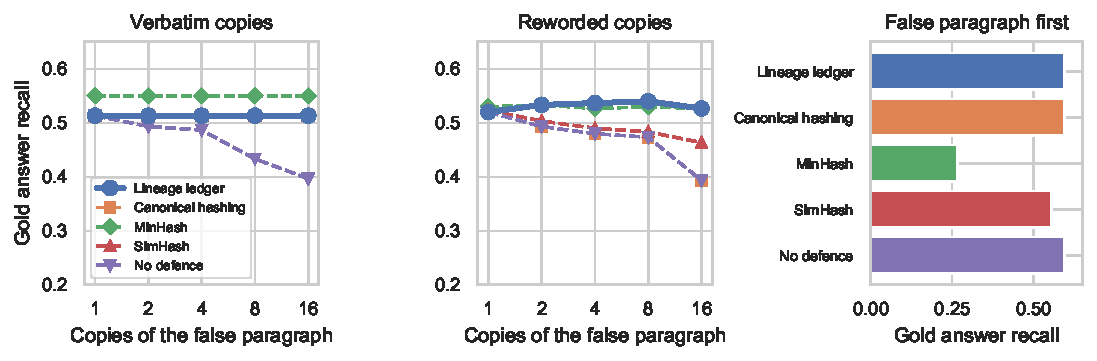
\includegraphics[width=\textwidth]{figures/fig_syndication.pdf}
\caption{Gold-answer recall of a frozen Qwen2.5-7B-Instruct reader on $300$
two-hop MuSiQue records as one counterfactual paragraph is repeated, after the
true paragraphs verbatim (left) and reworded (centre), and before them (right).
MinHash suppresses whichever of the true and false paragraphs arrives second. The ledger is the only
arm whose recall falls in no condition.}
\label{fig:syndication}
\end{figure}

Without a defence the reader follows the copies. Its gold-answer recall falls
from $\SyndPlainOne$ with one copy to $\SyndPlainSixteen$ with sixteen, a paired
change of $\SyndDrop$, interval $\SyndDropCI$, while the rate at which it
reports the planted answer rises from $\SyndMisledOne$ to $\SyndMisledSixteen$.
The decline is monotone in the number of copies, which extends the
majority-following of \citet{xie2024chameleon} to manufactured majorities.

Reading from the ledger removes the effect. All copies share one identifier, so
the reader sees the counterfactual once at every multiplicity. At sixteen copies
the ledger improves gold recall by $\SyndGain$, interval $\SyndGainCI$,
recovering the entire loss, and its context stays at $\SyndLedgerTokens$ tokens
against $\SyndPlainTokens$, a $\SyndTokenRatio$-fold reduction. All five
pre-registered predictions hold.

\begin{table}[t]
\centering\small
\caption{Frozen-reader results under syndicated misinformation, $300$ two-hop
MuSiQue records, Qwen2.5-7B-Instruct. Gold is gold-answer recall and misled is
the rate of reporting the planted answer. \emph{Truth kept} is the fraction of
records whose true final paragraph survives the rule, \emph{worst case} the
lowest gold recall of the three conditions, and tokens the mean context length
at sixteen verbatim copies.}
\label{tab:syndication}
\resizebox{\textwidth}{!}{%
\begin{tabular}{lcccccccc}
\toprule
& \multicolumn{2}{c}{Verbatim, $\times 16$} & \multicolumn{2}{c}{Reworded, $\times 16$} & \multicolumn{2}{c}{False first, $\times 1$} & & \\
\cmidrule(lr){2-3}\cmidrule(lr){4-5}\cmidrule(lr){6-7}
Accounting rule & Gold & Misled & Gold & Misled & Gold & Truth kept & Worst case & Tokens \\
\midrule
% generated by analysis/story_tables.py
\textbf{Lineage ledger (this work)} & $0.5133$ & $0.0100$ & $0.5267$ & $0.0133$ & $0.5967$ & $1.0000$ & $\mathbf{0.5133}$ & $464.5$ \\
Canonical hashing \citep{lee2022deduplicating} & $0.5133$ & $0.0100$ & $0.3933$ & $0.1533$ & $0.5967$ & $1.0000$ & $0.3933$ & $464.5$ \\
MinHash \citep{broder1997resemblance} & $0.5500$ & $0.0033$ & $0.5267$ & $0.0167$ & $0.2667$ & $0.4767$ & $0.2667$ & $386.3$ \\
SimHash \citep{charikar2002simhash, manku2007nearduplicate} & $0.5133$ & $0.0100$ & $0.4633$ & $0.0967$ & $0.5567$ & $0.9533$ & $0.4633$ & $454.4$ \\
No defence & $0.3967$ & $0.1367$ & $0.3933$ & $0.1533$ & $0.5967$ & $1.0000$ & $0.3933$ & $2362.1$
\\
\bottomrule
\end{tabular}}
\end{table}

\subsection{Surface similarity is not lineage}
\label{sec:surface}

Table~\ref{tab:syndication} shows why near-duplicate detection, the deployed
defence, cannot substitute for lineage. Canonical hashing
\citep{lee2022deduplicating} removes byte-identical copies and nothing else, so
once each copy carries its own outlet framing it behaves like no defence and
the ledger leads it by $\SyndCanonBoiler$ in gold recall, interval
$\SyndCanonBoilerCI$, changing the misled rate by $\SyndCanonBoilerMisled$.
SimHash \citep{charikar2002simhash} at the published radius
\citep{manku2007nearduplicate} catches some reworded copies and trails by
$\SyndSimBoiler$, interval $\SyndSimBoilerCI$.

MinHash \citep{broder1997resemblance} fails more consequentially. The
counterfactual differs from the true paragraph only in the answer span, so
MinHash judges them near-duplicates and keeps whichever arrives first. When the
false one arrives first it retains the true paragraph in only
$\SyndMinhashTrueKept$ of records, and from a single copy the ledger leads it by
$\SyndMinhashFirst$, interval $\SyndMinhashFirstCI$, and by
$\SyndMinhashFirstBoiler$ under reworded framing. A near-duplicate detector
cannot separate a copy from a contradiction, because the two differ only in
lineage. The ledger discards no lineage-distinct source, and its worst-case
recall in Table~\ref{tab:syndication} is the highest of any rule.

\subsection{Corroboration is directional}
\label{sec:directional}

Section~\ref{sec:conf} argues that a source should be credited only along the
directions its observation constrains. The real-data test asks whether that
predicts something a retrieval system must know before it answers, namely
whether the five retrieved MuSiQue paragraphs contain every supporting fact.
Table~\ref{tab:directional} reports the pre-registered comparison over
$\DirReN$ questions, of which $\DirReSufficient$ have sufficient evidence.

\begin{table}[t]
\centering\small
\caption{Predicting whether five retrieved MuSiQue paragraphs contain every
supporting paragraph, $\DirReN$ questions, AUROC within hop-count strata, the
pre-registered primary measure. Rows fix how lineage-distinct sources combine
within a requirement (Section~\ref{sec:conf}), and columns how requirements
combine. The first row is the pre-registered contrast. The second was
registered as a baseline, and its directional cell is the strongest score. Hop
count alone, with pooled AUROC $\DirReHopsPooled$, is constant within a
stratum. Appendix~\ref{app:directional} reports pooled values and copies.}
\label{tab:directional}
\begin{tabular}{lcc}
\toprule
& Weakest requirement & Mean requirement \\
Within a requirement & (directional) & (scalar) \\
\midrule
Sum over sources, registered primary & $\DirReDStrat$ & $\DirReSStrat$ \\
Best single source & $\mathbf{\DirReBestMinStrat}$ & $\DirReMeanBestStrat$ \\
\midrule
Sum of retrieval scores, no requirements & \multicolumn{2}{c}{$\DirReSumCosStrat$} \\
Best retrieval score, no requirements & \multicolumn{2}{c}{$\DirReMaxCosStrat$} \\
\bottomrule
\end{tabular}
\end{table}

Keeping requirements separate is what makes support informative. In the
pre-registered contrast, the weakest requirement's support exceeds the same
support averaged over requirements by $\DirReROne$ in stratified AUROC,
interval $\DirReROneCI$, and the averaged form is at chance within every hop
count, because a question can have many relevant sources and still no support
for one of its hops. When four copies of the top paragraph are appended, the
lineage-aware directional score exceeds provenance-free scalar counting by
$\DirReRTwo$, interval $\DirReRTwoCI$. Both pre-registered real-data
predictions hold, and the retrieval scores that systems commonly report, which
ignore requirements, fall well below every directional score.

The strongest score keeps each requirement's best single source, and it is
also directional, exceeding its own average over requirements by
$\DirReBestVsMean$, interval $\DirReBestVsMeanCI$, in an exploratory contrast.
Summed support trails it by $\DirReDvsBestMin$, interval $\DirReDvsBestMinCI$,
because sufficiency is a coverage question. A requirement is met once one
passage states it, so a second lineage-distinct passage cannot change the
label. Summation measures corroboration, which this
label does not reward, and it treats a related passage's partial projection as
a partial measurement. The best-source rule in turn cannot register a second
source at all, so where corroboration matters the additive join is needed, and
the ledger is what lets it credit a second source while ignoring a second copy.

\subsection{Conservation in a learned memory}
\label{sec:learned}

Table~\ref{tab:learned} reports a learned two-hop MuSiQue memory in three
regimes, scored by a content readout that does not depend on how credit is
scaled.

\begin{table}[t]
\centering\small
\caption{Learned two-hop MuSiQue memory at sixteenfold delivery, five seeds,
content readout, top-1 accuracy over $555$ candidate answers, where a uniform
guess scores $0.0018$. \emph{Re-chunked} delivers each paragraph with fifteen
windows cut from it, and \emph{fragments} delivers sixteen windows and
withholds the paragraph. Credit is relative to the lineage-distinct ceiling.
Appendix~\ref{app:duplication} gives fourfold delivery, NLL and MRR.}
\label{tab:learned}
\resizebox{\textwidth}{!}{%
\begin{tabular}{lccccc}
\toprule
Accounting rule & Clean & Exact & Re-chunked & Fragments & Credit, fragments \\
\midrule
% generated by analysis/learned_memory_table.py
\textbf{Lineage ledger (this work)} & $0.1141$ & $0.1141$ & $0.1141$ & $0.0832$ & $1.000$ \\
Canonical hashing \citep{lee2022deduplicating} & $0.1141$ & $0.1141$ & $0.0815$ & $0.0768$ & $16.000$ \\
MinHash \citep{broder1997resemblance} & $0.1141$ & $0.1141$ & $0.0816$ & $0.0851$ & $3.895$ \\
SimHash \citep{charikar2002simhash} & $0.1141$ & $0.1141$ & $0.0791$ & $0.0819$ & $11.849$ \\
Embedding detection \citep{xiao2023bge} & $0.1141$ & $0.1141$ & $0.0834$ & $0.0823$ & $5.588$ \\
No defence & $0.1141$ & $0.0823$ & $0.0815$ & $0.0768$ & $16.000$
\\
\bottomrule
\end{tabular}}
\end{table}

Under exact redelivery the ledger holds its clean accuracy of $\LmLedgerClean$,
because a redelivered hop is dropped before it reaches the recurrent content
path, while the provenance-free control processes every copy and falls to
$\LmPlainExactSixteen$. The ledger leads it by $\LmExactAccGain$, interval
$\LmExactAccGainCI$, changes negative log-likelihood by $\LmExactNllGain$ nats
and raises mean reciprocal rank by $\LmExactMrrGain$, every interval excluding
zero. Exact and near-duplicate matching equal the ledger here, since
byte-identical copies are what they catch.

Re-chunking separates what lineage does for accuracy from what it does for
credit. When a paragraph arrives together with windows cut from it, as in an
index that holds a document and its chunks, the ledger keeps the complete
rendering, since every window ranks below it, and every other rule loses more
than a quarter of its accuracy. The ledger leads no defence by
$\LmRechunkAccGain$, interval $\LmRechunkAccGainCI$, and the strongest
detector, \LmRechunkBestDetector, by $\LmRechunkDetGain$, interval
$\LmRechunkDetGainCI$. When only windows arrive, the ledger can hold only a
fragment, and as predicted before the run its accuracy is within noise of
reading every fragment, a difference of $\LmFragAccGain$ with interval
$\LmFragAccGainCI$, and of the strongest detector, \LmFragBestDetector, while it
credits one source where no defence credits sixteen. Lineage therefore always
bounds credit, and it also protects accuracy whenever a complete rendering of
the source is among the copies.

\subsection{Transfer and efficiency}
\label{sec:transfer}

The ledger attaches without modification to a message-passing backbone
\citep{gilmer2017mpnn}, a neural cellular automaton
\citep{mordvintsev2020growing} and a Set Transformer
\citep{lee2019settransformer}, conserving on each while the provenance-free
variants track the delivery count. It costs less than no defence, since
suppressed arrivals never reach the content path, running $4{,}674$ messages in
$0.037$ seconds against $0.063$, and under benign sixteenfold redelivery a
frozen Qwen2.5-1.5B-Instruct reader's context stays at
$\ReaderLedgerExactTokens$ tokens against $\ReaderPlainExactTokens$ with recall
unchanged (Appendices~\ref{app:fusion} and~\ref{app:transfer}).

\section{Limitations}
\label{sec:limits}

Source identity is not source truth. Nothing here discharges the assumption
of Section~\ref{sec:arrival} that a supplied identifier corresponds to a
distinct observation, and Proposition~\ref{prop:indist} shows content alone
cannot. Eight
machine paraphrases carrying fabricated identifiers inflate credited evidence
by $2.673$, which Appendix~\ref{app:sybil} records as a quantified boundary
rather than as Sybil robustness.

The frozen-reader results have two boundaries. When the true paragraph arrives
first, MinHash suppresses the counterfactual as a near-duplicate of it, and the
ledger minus MinHash difference is $\SyndMinhashLast$, interval
$\SyndMinhashLastCI$, the same order dependence that produces its deficit in
the reverse order. When sixteen copies precede the truth, the ledger changes the
misled rate by $\SyndFirstPlainMisled$, interval $\SyndFirstPlainMisledCI$, and
gold recall by $\SyndFirstPlainGold$, whose interval $\SyndFirstPlainGoldCI$
includes zero. Under benign duplication the arms
are indistinguishable on quality, so the benefit there is efficiency.

On AVeriTeC no variant separates on the official retrieved-track metric, and a
pre-registered selective-prediction criterion returned a negative decision, a
macro-F1 gain of $+0.0361$ with interval $[-0.0058, +0.0811]$. The learned
models carry roughly $0.5$M trainable parameters over a frozen $109$M encoder,
so larger scales remain to be measured.

The mechanism inherits the lineage its identifiers carry and trusts the version
a sender asserts. URL-level identifiers do not group a story syndicated across
outlets (Appendix~\ref{app:sybil}), and a sender who reuses a true source's
identifier with a higher refinement level can replace its content at unchanged
credit, so adversarial settings need versions authenticated by the issuer.

The directional evidence is real-data evidence only. In a synthetic learned
model, directional credit did not beat a scalar whose scale is learned, so two
of three registered synthetic predictions failed and no synthetic directional
claim is made (Appendix~\ref{app:directional}). The real-data test uses the
dataset's question decomposition as its requirement directions, which stands in
for a decomposer, and its strongest score was registered as a baseline rather
than as the primary.

\section{Conclusion}
\label{sec:conclusion}

Repetition is not corroboration, and corroboration has a direction. A memory
that credits lineage-distinct sources, each only along what it observed,
shields a frozen reader from a falsehood copied sixteen times without the order
dependence that makes near-duplicate detection discard the truth, tells when
retrieved evidence leaves a requirement unsupported, and keeps a learned
memory's accuracy under redelivery, with a finite-sample guarantee.

\label{endofmain}

\subsection*{AI use statement}

Generative tools were used in two distinct roles, and the roles are
distinguished because only one affects a reported number. As objects of study,
open models at pinned revisions served as frozen readers and produced the
paraphrase candidates for the Sybil audit, and Appendix~\ref{app:repro}
specifies their revisions and decoding settings. As a tool, an assistant
supported implementation, experimental design, interpretation and prose
revision. Automated tests check implementation properties and do not replace
author review of proofs or claims. The authors are responsible for the final
content, claims and artifacts.

\subsection*{Ethics statement}

This work uses two public research datasets and involves no human subjects.
AVeriTeC is used under its released licence and is not redistributed, and
MuSiQue is used and redistributed under CC BY 4.0. The counterfactual
paragraphs are generated mechanically from public records, are framed with
generic outlet labels rather than real organisations, and are released only as
evaluation artifacts. Section~\ref{sec:limits} reports an attack that fabricates
source identity, because a defence whose failure mode is quantified is safer
than one whose failure mode is undocumented. A mechanism that bounds confidence
could be misread as a guarantee of correctness. The guarantee is that credited
evidence does not grow under repetition of a stable lineage, and it says nothing
about whether the underlying source is true.

\subsection*{Reproducibility statement}

Every number reported here is read from a committed raw output. The
syndication, reader, directional, learned-memory and taxonomy numbers are
written by the scripts listed in Appendix~\ref{app:repro}, and the remaining
numbers are transcribed from the committed reports named there. The theoretical claims are
stated with their assumptions in Appendix~\ref{app:theory}, and every proof
appears there in full. Appendix~\ref{app:repro} records the hardware, the pinned
revisions, the seed counts, the parameter counts and the regeneration commands.
The syndication and directional experiments were pre-registered before any
output existed, and Appendices~\ref{app:syndication} and~\ref{app:directional}
report their predictions and decision rules. The MuSiQue corpus ships compressed in the repository with a digest
manifest. AVeriTeC is not redistributed, and the official knowledge store is
used in place of live web search. The full source, including the test suite
that guards the structural properties asserted here, is available
anonymously.\footnote{Anonymised code and data:
\url{ANONYMOUS-CODE-URL-TO-BE-INSERTED}. The repository contains the committed
raw outputs, the analysis scripts that produce every table and figure, and the
pre-registration document.}

\label{endofstatements}
\bibliographystyle{iclr2027_conference}
\bibliography{refs}

\clearpage
\appendix

\section{Assumptions and complete proofs}
\label{app:theory}

This appendix states the assumptions behind Theorem~\ref{thm:categorical},
gives its formal statement and proof, proves Corollary~\ref{cor:invariance},
states and proves Proposition~\ref{prop:directional} in full, and establishes
the two propositions on calibration and on lineage used in the main text.

\subsection{Assumptions}

Each assumption is stated where it is first used, and the scope of every
statement below is limited to the assumptions it names.

\begin{assumption}[Lipschitz readout]
\label{ass:readout}
The decoder $g$ maps a normalized ledger summary $h$ and a mass $W$ to logits,
and satisfies
$\|g(h',W')-g(h,W)\|_\infty\le L_h\|h'-h\|_2+L_W|W'-W|$ with constants that do
not depend on the delivery count.
\end{assumption}

\begin{assumption}[Stable lineage]
\label{ass:lineage}
Root identifiers are assigned by an oracle and are not under adversarial
control. Proposition~\ref{prop:indist} shows why this cannot be replaced by an
inference from content.
\end{assumption}

\begin{assumption}[Independent coordinated hashing]
\label{ass:hash}
Root hashes $u_r=h(r)$ are independent and uniform on $[0,1)$, and the payloads
and weights are fixed given the root set, so the retained subset is independent
of the values it retains. The implementation approximates this idealization
with a seeded $64$-bit digest.
\end{assumption}

\subsection{Formal statement of Theorem~\ref{thm:categorical}}

Fix root payloads $a_r\in\mathbb R^p$ and weights $w_r>0$ independently of the
sketch hashes. Write $W=\sum_r w_r$ and $h=\sum_r a_r/W$. A coordinated
bottom-$k$ sample $I$ with cardinality budget $k_h\ge k$ defines
\[
\hat h=\frac{\sum_{r\in I}a_r}{\sum_{r\in I}w_r},\qquad
\hat W=\frac{\hat n}{|I|}\sum_{r\in I}w_r.
\]
Let $q=\operatorname{softmax}g(h,W)$ and
$\hat q=\operatorname{softmax}g(\hat h,\hat W)$ under
Assumption~\ref{ass:readout}. For $\delta\in(0,1)$ the finite-population radii
$r_h$ and $r_W$ of Equation~\ref{eq:categorical-radii} are functions of
$(n,k,k_h,\{a_r,w_r\},\delta)$. When the denominator condition $e<1$ holds, with
probability at least $1-\delta$, putting $A=L_h r_h+L_W r_W$ gives
\begin{equation}
\mathrm{KL}(q\,\|\,\hat q)\le A^2/2,\qquad
|{-\log\hat q_y}+\log q_y|\le2A\quad\text{for every label }y.
\label{eq:categorical-memory}
\end{equation}
An exact-readout top-two logit margin greater than $2A$ guarantees the same
predicted class. For $n\le k$ all radii are zero. Replaying held versions
changes neither readout nor the bound.

\subsection{Proof of Theorem~\ref{thm:categorical}}

\paragraph{Radii.}
Put $u_r=a_r-w_rh$, so that $\sum_ru_r=0$, and define
\begin{align}
c&=\begin{cases}n(n-k)/[k(n-1)]&n>k,\\0&n\le k,\end{cases}\nonumber\\
V_u&=c\sum_r\|u_r\|_2^2,\qquad
V_D=c\sum_r(w_r-W/n)^2,\qquad V_M=\mathrm{Var}(\hat W).
\label{eq:categorical-moments}
\end{align}
The mass variance $V_M$ is finite when cardinality is exact or $k_h\ge2$. For a
chosen failure probability define
\begin{equation}
e=\frac{\sqrt{3V_D/\delta}}{W},\quad
r_h=\frac{\sqrt{3V_u/\delta}}{W(1-e)},\quad
r_W=\sqrt{3V_M/\delta},\qquad e<1.
\label{eq:categorical-radii}
\end{equation}
When $e\ge1$ the bound is vacuous. The radii use the full population, so they
are conditional analytic bounds rather than certificates computable from a
sketch alone. Because $e$ is a Chebyshev radius, the denominator condition
constrains the retained fraction $k/n$, and the bound is informative under mild
compression.

\paragraph{Sampling step.}
For $n>k$, bottom-$k$ selects a uniform $k$-subset independently of the ordered
hash values. With $\tilde U=(n/k)\sum_Iu_r$ and $\tilde D=(n/k)\sum_Iw_r$, the
simple-random-sampling moments are
\[
\mathbb E\tilde U=0,\quad \mathbb E\|\tilde U\|_2^2=V_u,\quad
\mathbb E\tilde D=W,\quad \mathrm{Var}(\tilde D)=V_D.
\]
Subset indicators satisfy $\mathbb EI_r=k/n$ and
$\mathbb EI_rI_s=k(k-1)/[n(n-1)]$. Expanding the squared norm and using
$\sum_ru_r=0$ gives $V_u$, and centering $w_r$ gives $V_D$. Markov's inequality
on $\|\tilde U\|_2^2$ and Chebyshev's inequality on $\tilde D$ and $\hat W$,
each with failure probability $\delta/3$, give simultaneously
$\|\tilde U\|_2\le\sqrt{3V_u/\delta}$, $\tilde D\ge W(1-e)$ and
$|\hat W-W|\le r_W$. The union bound requires no independence between these
events. Since $\hat h-h=\tilde U/\tilde D$, it follows that
$\|\hat h-h\|_2\le r_h$. The case $n\le k$ is exact.

\paragraph{Neural and categorical steps.}
Let $z=g(h,W)$ and $v=g(\hat h,\hat W)-z$. Assumption~\ref{ass:readout} gives
$\|v\|_\infty\le A$ on the same event. For $q=\operatorname{softmax}z$, direct
substitution gives
\begin{equation}
\mathrm{KL}(q\,\|\,\hat q)=\log\mathbb E_{j\sim q}e^{v_j}-\mathbb E_{j\sim q}v_j
\le\frac{(\max_jv_j-\min_jv_j)^2}{8}\le\frac{A^2}{2},
\end{equation}
where the first inequality is Hoeffding's lemma
\citep{hoeffding1963probability}. For each label the loss change is
$\log\mathbb E_q e^{v_j}-v_y$. Both terms lie between $\min_jv_j$ and
$\max_jv_j$, so its absolute value is at most $2A$. A top-two margin greater
than $2A$ cannot be reversed by coordinate changes of magnitude at most $A$,
which proves all three claims.

\paragraph{Scope.}
A decoder of the form $g(h,W)=A_2\tanh(A_1h+b_1)+b_2+vW$ admits
$L_h\le\|A_2\|_{2\to\infty}\|A_1\|_2$ and $L_W=\|v\|_\infty$, so the interface
admits nonlinear neural computation. Because $\hat n$ cancels from $\hat h$,
extra hash slots improve mass estimation but cannot repair content error when
$L_W=0$. The bound compares two model distributions rather than either model
with the true conditional, and it applies to a fixed population rather than to
populations chosen adaptively in response to the hashes. $\blacksquare$

\subsection{Proof of Corollary~\ref{cor:invariance}}

\begin{proof}
Let the ledger $L$ contain root $r$ at version $v$. Delivering $r$ again at any
version $v'$ replaces the entry with $\arg\max_\kappa\{v,v'\}$. If $v'=v$ the
result is $v$ by idempotence. If $\rho_{v'}<\rho_v$ then $v$ wins outright. If
$\rho_{v'}=\rho_v$ the $-m$ coordinate ensures that a version claiming greater
mass cannot displace the incumbent. In every such case the ledger is unchanged
as a value, so the credited quantity $\rho_{ir}\Lambda_r$ in
Equation~\ref{eq:psd} and every downstream readout are unchanged. The joins are
commutative and associative, so the conclusion holds for any order and any
number of such deliveries. If instead $\kappa(v')>\kappa(v)$, the domain of the
ledger is unchanged because $r$ was already present, so credited evidence is
unchanged and only the representation moves. Credit therefore depends on the
number $R$ of roots in the domain and not on the number $N$ of arrivals.
\end{proof}

\subsection{Unbiasedness of the Horvitz-Thompson readout}

Let root $r$ carry the additive payload $\eta_r$, so the quantity to estimate
is $S=\sum_r\eta_r$ over $n>k$ roots.

\begin{proof}
Under Assumption~\ref{ass:hash} the sketch retains the $k$ roots with the
smallest hashes, and $\theta=u_{(k+1)}$ is the $(k+1)$st smallest hash. The
argument conditions on ranks rather than on $\theta$, since given $\theta$
exactly $k$ roots fall below it and inclusions are not independent
\citep{cohen2007bottomk}. For a fixed root $r$, let $\tau_r$ be the $k$th
smallest hash among the other $n-1$ roots. Then $r$ is retained if and only if
$u_r<\tau_r$, and whenever it is retained $\theta=\tau_r$, because $r$ is then
one of the $k$ smallest and the $(k+1)$st smallest overall is the $k$th smallest
of the rest. The estimator therefore gives root $r$ the weight
$\mathbf{1}\{u_r<\tau_r\}/\tau_r$. Since $\tau_r$ depends only on the other
hashes, it is independent of $u_r$, and
$\mathbb{E}[\mathbf{1}\{u_r<\tau_r\}/\tau_r\mid\tau_r]=1$. Summing over roots
gives $\mathbb{E}[\hat S]=\sum_r\eta_r=S$.
\end{proof}

\subsection{Formal statement and proof of Proposition~\ref{prop:directional}}

Let the ledger hold $n$ roots, root $r$ at a version whose credited precision
is $M_r=\rho_{ir}\Lambda_r\succeq0$, and let
$\Lambda=\Lambda_{\text{prior}}+\sum_rM_r$ as in Equation~\ref{eq:psd}. For a
unit vector $u$ the support is $s(u)=u^\top\Lambda u$. For unit requirement
directions $d_1,\dots,d_H$ the directional confidence is
$\gamma=\min_hs(d_h)$, and its conservative form, which keeps the best single
source per requirement, is
$\gamma^\vee=\min_h\bigl(d_h^\top\Lambda_{\text{prior}}d_h+\max_rd_h^\top
M_rd_h\bigr)$. The scalar surrogate is
$\Lambda^{\mathrm{sc}}=\Lambda_{\text{prior}}+\sum_r\tfrac{1}{d}\mathrm{tr}(M_r)I$.

\paragraph{Statement.} (i) $\Lambda$, $\gamma$ and $\gamma^\vee$ are functions
of the ledger state, so they are unchanged by any permutation of arrivals and
by any redelivery of a held version, and they depend on the $R$ held roots and
not on the $N\ge R$ arrivals. (ii) If $M_ru=0$ for every $r$, then
$s(u)=u^\top\Lambda_{\text{prior}}u$, whereas
$\mathrm{tr}\,\Lambda^{\mathrm{sc}}=\mathrm{tr}\,\Lambda$ and
$u^\top(\Lambda^{\mathrm{sc}}-\Lambda_{\text{prior}})u=\tfrac{1}{d}\sum_r
\mathrm{tr}(M_r)$ for every unit $u$, which is positive unless every $M_r$
vanishes. Under an isotropic prior the surrogate's weakest-requirement
confidence is therefore the same for every set of requirements. (iii) Let $I$ be
a coordinated bottom-$k$ sample of the $n>k$ roots under
Assumption~\ref{ass:hash}, with the cardinality $n$ known, and put
$\hat\Lambda=\Lambda_{\text{prior}}+\tfrac{n}{k}\sum_{r\in I}M_r$. Then
$\mathbb{E}\hat\Lambda=\Lambda$, and with probability at least $1-\delta$
\begin{equation}
\sup_{\|u\|_2=1}\bigl|\hat s(u)-s(u)\bigr|\le\|\hat\Lambda-\Lambda\|_2\le
r_\Lambda=\sqrt{V_\Lambda/\delta},\qquad
V_\Lambda=c\sum_r\|M_r-\bar M\|_F^2,
\label{eq:directional-radius}
\end{equation}
with $c$ as in Equation~\ref{eq:categorical-moments} and
$\bar M=\tfrac{1}{n}\sum_rM_r$, so that $|\hat\gamma-\gamma|\le r_\Lambda$ on the
same event. For rank-one credit $M_r=\rho_re_re_r^\top$ with $\|e_r\|_2=1$ and
$\rho_r\le1$, $r_\Lambda\le n\sqrt{(n-k)/(k(n-1)\delta)}$. For $n\le k$ the
sketch is exact. An estimated cardinality adds its own variance, as the term
$V_M$ does in Theorem~\ref{thm:categorical}. (iv) The conservative confidence
computed on the sample satisfies $\hat\gamma^\vee\le\gamma^\vee$ with
probability one.

\begin{proof}
(i) By Corollary~\ref{cor:invariance}, a redelivery that does not beat the
incumbent leaves the ledger unchanged as a value, and the joins are commutative
and associative, so every arrival order and every number of such redeliveries
reach one ledger state. $\Lambda$, $\gamma$ and $\gamma^\vee$ read only the held
versions. A strictly better version replaces $M_r$ for a root already held and
leaves the number of summands at $R$.

(ii) $s(u)-u^\top\Lambda_{\text{prior}}u=\sum_ru^\top M_ru=0$ when every
$M_ru=0$. The trace is linear and
$\mathrm{tr}\bigl(\tfrac{1}{d}\mathrm{tr}(M_r)I\bigr)=\mathrm{tr}(M_r)$. For
unit $u$, $u^\top\bigl(\tfrac{1}{d}\mathrm{tr}(M_r)I\bigr)u=\tfrac{1}{d}
\mathrm{tr}(M_r)$, and a nonzero positive semidefinite matrix has positive
trace. With $\Lambda_{\text{prior}}=\lambda I$ the surrogate gives every
requirement the support $\lambda+\tfrac{1}{d}\sum_r\mathrm{tr}(M_r)$.

(iii) Put $x_r=\mathrm{vec}(M_r)$ and $y_r=x_r-\bar x$, so $\sum_ry_r=0$ and,
since $\tfrac{n}{k}\sum_{r\in I}\bar x=\sum_rx_r$,
$\mathrm{vec}(\hat\Lambda-\Lambda)=\tfrac{n}{k}\sum_{r\in I}y_r$. As in the
proof of Theorem~\ref{thm:categorical}, $I$ is a uniform $k$-subset independent
of the payloads, with $\mathbb{E}I_r=k/n$ and
$\mathbb{E}I_rI_s=k(k-1)/[n(n-1)]$. Hence $\mathbb{E}\hat\Lambda=\Lambda$, and
using $\sum_{r\ne s}y_r^\top y_s=-\sum_r\|y_r\|_2^2$,
\[
\mathbb{E}\Bigl\|\tfrac{n}{k}\textstyle\sum_{r\in I}y_r\Bigr\|_2^2
=\tfrac{n^2}{k^2}\Bigl(\tfrac{k}{n}-\tfrac{k(k-1)}{n(n-1)}\Bigr)
\textstyle\sum_r\|y_r\|_2^2=c\sum_r\|y_r\|_2^2=V_\Lambda .
\]
Markov's inequality on $\|\hat\Lambda-\Lambda\|_F^2$ gives
$\|\hat\Lambda-\Lambda\|_F\le r_\Lambda$ with probability at least $1-\delta$.
For a symmetric matrix $A$ and unit $u$,
$|u^\top Au|\le\|A\|_2\le\|A\|_F$, and
$|\min_ha_h-\min_hb_h|\le\max_h|a_h-b_h|$ transfers the bound to $\gamma$. For
rank-one credit, $\sum_r\|y_r\|_2^2\le\sum_r\|x_r\|_2^2=\sum_r\rho_r^2\le n$, so
$V_\Lambda\le cn=n^2(n-k)/[k(n-1)]$.

(iv) For each $h$, a maximum over the retained roots cannot exceed the maximum
over all roots, and taking the minimum over $h$ preserves the inequality.
\end{proof}

Part (ii) makes precise the claim of Section~\ref{sec:conf} that a scalar count
keeps the total information and discards its direction. Part (iii) is the
directional analogue of the representation radius of
Theorem~\ref{thm:categorical}, and like it the radius involves only the held
roots.

\subsection{The calibration penalty of over-counted precision}

\begin{proposition}[Calibration penalty]
\label{prop:calibration}
Let one underlying observation of precision $\Lambda$ be delivered $N$ times,
and let a provenance-free readout credit every arrival, so that it reports
precision $N\Lambda$ where the correct posterior carries $\Lambda$. For
$d$-dimensional Gaussian posteriors sharing a mean, the divergence from the
correct posterior to the reported one is
\begin{equation}
\mathrm{KL}(N) \;=\; \tfrac{d}{2}\bigl(N - 1 - \ln N\bigr),
\label{eq:klpenalty}
\end{equation}
which vanishes at $N=1$ and grows without bound. A conserving readout reports
$\Lambda$ at every $N$, so its divergence under the same model is zero.
\end{proposition}

\begin{proof}
For Gaussians with a common mean and precisions $\Lambda$ and $N\Lambda$, the
divergence is
\[
\tfrac{1}{2}\bigl(\mathrm{tr}(N\Lambda\Lambda^{-1}) - d
- \ln\det(N\Lambda\Lambda^{-1})\bigr)
= \tfrac{1}{2}(Nd - d - d\ln N),
\]
which is Equation~\ref{eq:klpenalty}.
Non-negativity and monotonicity on $N \geq 1$ follow because the derivative
$\tfrac{d}{2}(1 - 1/N)$ is non-negative there.
\end{proof}

Equation~\ref{eq:klpenalty} states the scale of the cost of over-counting in
the idealised case the proposition names. A learned model violates its shared
mean premise, because its predicted mean also moves with the evidence it is
given, so the expression is used here as a statement of scale and not as a
prediction of any measured quantity.

\subsection{Content does not determine lineage}

\begin{proposition}[Indistinguishability]
\label{prop:indist}
There exist two generative processes, one emitting $m$ copies of a single
observation and one emitting $m$ separately acquired observations, that induce
identical distributions over the visible content. No function of content alone
distinguishes them, so any accounting rule that reads content only must either
over-credit the first process or under-credit the second.
\end{proposition}

\begin{proof}
Let a source emit a fixed value $v$ almost surely. Process A draws once from
one such source and copies the result $m$ times. Process B draws once from each
of $m$ distinct such sources. Both produce the content multiset $\{v\}^m$ with
probability one, so the induced distributions over visible content are equal
and no measurable function of content separates them. Evidence conservation
must credit A once and B $m$ times, so a content-only rule that is correct on A
is wrong on B and conversely.
\end{proof}

The syndication experiment exhibits the converse direction of the same fact. A
counterfactual that edits one span of a true paragraph shares almost all of its
content yet descends from a different source, and Section~\ref{sec:surface}
shows what a content-only rule does with it.

\section{Syndication experiment in full}
\label{app:syndication}

This appendix reproduces the pre-registered design, reports the outcome of
every prediction, and tabulates every condition. The pre-registration document
was committed to the repository before any reader call was made, and the
verdict below is computed from the per-record outputs by a script that applies
the committed decision rules mechanically.

\paragraph{Question and construction.} \citet{xie2024chameleon} report that
language models follow the side with more evidence when the supporting pieces
are distinct texts. The experiment asks whether a frozen reader treats copies of
one false source as additional evidence, and whether reading from the ledger
removes that exposure. A record is eligible only if no gold answer or alias
survives in the counterfactual, the substitute appears in it, and the
substitute appears in neither true paragraph. Substitutes match the kind of the
gold answer, whether a year, another number or an entity of similar length,
since an implausible substitute would be rejected on plausibility alone.
Reworded copies are framed as ``Outlet $k$ reports'' with a trailing
syndication marker, so no two copies share bytes while all share one lineage.

\paragraph{Fixed in advance.} The reader is Qwen2.5-7B-Instruct
\citep{qwen2025qwen25} with greedy decoding and $48$ new tokens. The records
are the first $300$ eligible in file order, and no record was added after any
output was seen. Intervals use $10{,}000$ bootstrap resamples over records with
percentile bounds. A context-building pass with no reader loaded established
that MinHash and SimHash can suppress the counterfactual or the true paragraph
as near-duplicates of each other, which is why the order-dependence prediction
was registered.

\begin{table}[h]
\centering\small
\caption{Pre-registered predictions and their outcomes. Differences are paired
over the $300$ records. All $\SyndHeld$ of $\SyndPredictions$ predictions
hold.}
\label{tab:prereg}
\resizebox{\textwidth}{!}{%
\begin{tabular}{llcc}
\toprule
Prediction & Contrast & Difference & $95\%$ interval \\
\midrule
P1, the phenomenon & No defence, sixteen minus one verbatim copy, gold & $\SyndDrop$ & $\SyndDropCI$ \\
P2, protection & Ledger minus no defence, sixteen verbatim copies, gold & $\SyndGain$ & $\SyndGainCI$ \\
P3, misled rate rises & No defence, sixteen minus one verbatim copy, misled & $\SyndMisledRise$ & $\SyndMisledRiseCI$ \\
P4, hashing fails on rewording & Canonical hashing minus no defence, sixteen reworded copies, gold & $\SyndCanonPlain$ & $\SyndCanonPlainCI$ \\
P5, order dependence & Ledger minus MinHash, one copy before the truth, gold & $\SyndMinhashFirst$ & $\SyndMinhashFirstCI$ \\
\bottomrule
\end{tabular}}
\end{table}

Table~\ref{tab:prereg} lists the outcomes, and Table~\ref{tab:synd-full}
reports gold-answer recall in every condition. The ledger's verbatim rows are
constant across multiplicity by construction, since repeated copies of one root
are no-ops. The difference between the ledger and no defence at sixteen copies
therefore equals the amount by which repetition moves the reader.

\begin{table}[h]
\centering\small
\caption{Gold-answer recall in every syndication condition, $300$ records,
Qwen2.5-7B-Instruct.}
\label{tab:synd-full}
\resizebox{\textwidth}{!}{%
\begin{tabular}{llccccc}
\toprule
Accounting rule & Copies & $\times 1$ & $\times 2$ & $\times 4$ & $\times 8$ & $\times 16$ \\
\midrule
\multicolumn{7}{l}{\emph{False copies after the truth}} \\
% generated by analysis/story_tables.py
\textbf{Lineage ledger (this work)} & verbatim & $0.5133$ & $0.5133$ & $0.5133$ & $0.5133$ & $0.5133$ \\
\textbf{Lineage ledger (this work)} & reworded & $0.5200$ & $0.5333$ & $0.5367$ & $0.5400$ & $0.5267$ \\
Canonical hashing \citep{lee2022deduplicating} & verbatim & $0.5133$ & $0.5133$ & $0.5133$ & $0.5133$ & $0.5133$ \\
Canonical hashing \citep{lee2022deduplicating} & reworded & $0.5200$ & $0.4933$ & $0.4800$ & $0.4733$ & $0.3933$ \\
MinHash \citep{broder1997resemblance} & verbatim & $0.5500$ & $0.5500$ & $0.5500$ & $0.5500$ & $0.5500$ \\
MinHash \citep{broder1997resemblance} & reworded & $0.5300$ & $0.5333$ & $0.5267$ & $0.5300$ & $0.5267$ \\
SimHash \citep{charikar2002simhash, manku2007nearduplicate} & verbatim & $0.5133$ & $0.5133$ & $0.5133$ & $0.5133$ & $0.5133$ \\
SimHash \citep{charikar2002simhash, manku2007nearduplicate} & reworded & $0.5233$ & $0.5033$ & $0.4900$ & $0.4833$ & $0.4633$ \\
No defence & verbatim & $0.5133$ & $0.4933$ & $0.4867$ & $0.4333$ & $0.3967$ \\
No defence & reworded & $0.5200$ & $0.4933$ & $0.4800$ & $0.4733$ & $0.3933$
\\
\addlinespace
\multicolumn{7}{l}{\emph{False copies before the truth}} \\
% generated by analysis/story_tables.py
\textbf{Lineage ledger (this work)} & verbatim & $0.5967$ & $0.5967$ & $0.5967$ & $0.5967$ & $0.5967$ \\
\textbf{Lineage ledger (this work)} & reworded & $0.5767$ & $0.5667$ & $0.5700$ & $0.5700$ & $0.5733$ \\
Canonical hashing \citep{lee2022deduplicating} & verbatim & $0.5967$ & $0.5967$ & $0.5967$ & $0.5967$ & $0.5967$ \\
Canonical hashing \citep{lee2022deduplicating} & reworded & $0.5767$ & $0.4733$ & $0.5200$ & $0.5367$ & $0.5433$ \\
MinHash \citep{broder1997resemblance} & verbatim & $0.2667$ & $0.2667$ & $0.2667$ & $0.2667$ & $0.2667$ \\
MinHash \citep{broder1997resemblance} & reworded & $0.3767$ & $0.3667$ & $0.3667$ & $0.3700$ & $0.3667$ \\
SimHash \citep{charikar2002simhash, manku2007nearduplicate} & verbatim & $0.5567$ & $0.5567$ & $0.5567$ & $0.5567$ & $0.5567$ \\
SimHash \citep{charikar2002simhash, manku2007nearduplicate} & reworded & $0.5533$ & $0.4700$ & $0.4900$ & $0.5100$ & $0.4967$ \\
No defence & verbatim & $0.5967$ & $0.5200$ & $0.5767$ & $0.5867$ & $0.5733$ \\
No defence & reworded & $0.5767$ & $0.4733$ & $0.5200$ & $0.5367$ & $0.5433$
\\
\bottomrule
\end{tabular}}
\end{table}

\section{Directional credit experiments in full}
\label{app:directional}

Both experiments follow a pre-registration committed before any output
existed, together with two dated amendments that were also committed before any
output. The first amendment appended the copies in the real-data duplicated
condition to the retrieved set, because exact copies tie with their original
under cosine retrieval and would otherwise fill every slot and make the label
constant. The second followed an independent audit of the design. It added a
scalar arm whose overall scale is learned, which became the primary synthetic
comparator, and it stratified the primary real-data test by hop count and added
hop count, best-single-source and retrieval-score baselines, because the number
of decomposition steps equals the number of supporting paragraphs and hop count
alone predicts sufficiency. \path{analysis/directional_analysis.py} applies the
registered rules to the committed outputs.

\paragraph{Synthetic.} The task is the evidence graph of
Appendix~\ref{app:transfer}, with a four-dimensional latent, three roots, eight
cells on a path, eight message steps, $4{,}000$ training iterations and five
seeds. Sources observe one, two or four directions. Every arm shares one
content path. Directional credit uses each root's precision, the scalar arms
use $\tfrac{1}{d}\mathrm{tr}(\Lambda_r)I$, and the fitted scalar arm multiplies
that by a learned global scale. Table~\ref{tab:directional-synthetic} reports
the negative log-likelihood of the true latent. Directional credit has the
lowest error at every rank, but its registered advantage over the fitted scalar
at rank one, $\DirSynSOne$ nats with interval $\DirSynSOneCI$, does not exclude
zero, and the advantage grows rather than shrinks with rank, so the registered
predictions S1 and S3 fail and no synthetic directional claim is made. The
lineage prediction S2 holds, with $\DirSynSTwo$ nats, interval $\DirSynSTwoCI$.

\begin{table}[h]
\centering\small
\caption{Synthetic directional credit, five seeds. Negative log-likelihood of
the true latent under clean delivery at each observation rank, under sixteenfold
duplication at rank one, and coverage of the marginal $95\%$ interval at rank
one. The pre-registration named $90\%$ coverage as a secondary metric; the
coverage routine the model already used measures $95\%$, and that is what is
reported.}
\label{tab:directional-synthetic}
\resizebox{\textwidth}{!}{%
\begin{tabular}{lccccc}
\toprule
Credit & Rank 1 & Rank 2 & Rank 4 & Rank 1, $\times 16$ & $95\%$ coverage \\
\midrule
% generated by analysis/directional_analysis.py
\textbf{Lineage, directional (this work)} & $5.4535$ & $4.7639$ & $3.8581$ & $6.8171$ & $0.9184$ \\
Lineage, scalar with learned scale & $5.5639$ & $4.9065$ & $4.0863$ & $6.7580$ & $0.9094$ \\
Lineage, scalar & $5.7140$ & $5.1473$ & $4.4186$ & $7.1349$ & $0.8875$ \\
No lineage, directional & $5.4535$ & $4.7639$ & $3.8581$ & $28.6837$ & $0.9184$ \\
No lineage, scalar & $5.7140$ & $5.1473$ & $4.4186$ & $31.2987$ & $0.8875$
\\
\bottomrule
\end{tabular}}
\end{table}

\paragraph{Real data.} Paragraphs and queries are encoded with BGE
\texttt{bge-base-en-v1.5} \citep{xiao2023bge} at a pinned revision, with the
retrieval instruction applied to queries only. Intervals come from $10{,}000$
paired bootstrap resamples over records, resampled within hop strata for the
stratified tests. Table~\ref{tab:directional-musique} reports every score.
The best-single-source scores use the cosine rather than its square. Every
record's best cosine is at least $\DirReBestFloor$, so the two order records
identically, and the score is the rank-one support of the single best source,
the conservative form $\gamma^\vee$ of Appendix~\ref{app:theory}. The contrast
between its weakest and mean requirement was not registered and is reported as
exploratory. Pooled over hop counts, the best-source score reaches
$\DirReBestMinPooled$, above hop count alone at $\DirReHopsPooled$.

\begin{table}[h]
\centering\small
\caption{Predicting whether five retrieved MuSiQue paragraphs contain every
supporting paragraph. AUROC pooled over records and stratified by hop count,
and pooled AUROC with four copies of the top paragraph appended and counted per
arrival. Counted once per lineage, the copies leave every score at its clean
value by construction. Weakest-requirement rows are directional and
mean-requirement rows scalar.}
\label{tab:directional-musique}
\resizebox{\textwidth}{!}{%
\begin{tabular}{lccc}
\toprule
Score & Clean & Clean, stratified & Copies, per arrival \\
\midrule
% generated by analysis/directional_analysis.py
Weakest requirement, sum over sources (registered primary) & $0.6989$ & $0.6563$ & $0.6874$ \\
Mean requirement, sum over sources & $0.6019$ & $0.5028$ & $0.6508$ \\
Weakest requirement, best single source & $0.7404$ & $0.7132$ & $0.7404$ \\
Mean requirement, best single source & $0.7151$ & $0.6930$ & $0.7151$ \\
Sum of retrieval scores & $0.5006$ & $0.4671$ & $0.5633$ \\
Maximum retrieval score & $0.6137$ & $0.5467$ & $0.6137$ \\
Hop count alone & $0.7018$ & $0.5000$ & $0.7018$
\\
\bottomrule
\end{tabular}}
\end{table}

\section{Duplicated-hop construction}
\label{app:duplication}

The learned memory transports evidence along MuSiQue chains, one hop per
delivery, and each regime rewrites the delivery stream of a chain while keeping
the root identifier of every arrival. Every construction is deterministic, so
intervals come from seeds of the learned model rather than from randomness in
the stream. Table~\ref{tab:learned-full} reports every arm in every regime with
the readout and seeds of Table~\ref{tab:learned}.

\paragraph{Exact.} An arrival is repeated verbatim.

\paragraph{Re-chunked.} At multiplicity $m$ the paragraph arrives once in full
and then as $m-1$ distinct contiguous windows cut from it, with widths nearest
seventy percent of the paragraph and offsets spread across it, so no window adds
a fact and every window has its own surface hash. The windows at a lower
multiplicity are a prefix of those at a higher one. A window carries a subset of
its paragraph's content, so it ranks below the paragraph in the version key by
the number of words it omits. The ledger therefore holds the whole paragraph and
its content path sees exactly the clean stream, while credit, which counts
identifiers, is unaffected. Exact hashing admits every window as a new source,
the near-duplicate detectors admit those they do not judge similar to an
earlier arrival, and the provenance-free control processes all of them. The
detectors suppress some windows, as their credit in Table~\ref{tab:taxonomy}
shows, but the windows they admit move the content path about as far as all
sixteen renderings move the undefended memory.

\paragraph{Fragments.} The same windows arrive without the paragraph, $m$ of
them at multiplicity $m$, so no complete rendering exists and every rule,
the ledger included, can hold only a fragment. The two predictions, credit of
exactly one unit per source and an accuracy difference against no defence whose
interval includes zero at sixteenfold, were committed before any output of this
regime existed, and both hold. A window that outranks the one held replaces it
and reaches the content path, so at sixteenfold $\LmFragLedgerReach$ of
$\LmFragArrivals$ arrivals per record reach the ledger's content path, which is
why its accuracy is lower at sixteenfold than at fourfold. An earlier
fragments-only run with at most three distinct windows gave the same result, a
ledger minus no defence difference of $\LmOverlapAccGain$ with interval
$\LmOverlapAccGainCI$.

\begin{table}[h]
\centering\small
\caption{Learned two-hop MuSiQue memory in every duplication regime, five
seeds, content readout. Accuracy is top-1 over $555$ candidate answers, and
negative log-likelihood and mean reciprocal rank are at sixteenfold delivery.}
\label{tab:learned-full}
\resizebox{\textwidth}{!}{%
\begin{tabular}{lccccc}
\toprule
Accounting rule & Clean & $\times 4$ & $\times 16$ & NLL, $\times 16$ & MRR, $\times 16$ \\
\midrule
\multicolumn{6}{l}{\emph{Exact}} \\
% generated by analysis/learned_memory_table.py
\textbf{Lineage ledger (this work)} & $0.1141$ & $0.1141$ & $0.1141$ & $5.5337$ & $0.1986$ \\
Canonical hashing \citep{lee2022deduplicating} & $0.1141$ & $0.1141$ & $0.1141$ & $5.5337$ & $0.1986$ \\
MinHash \citep{broder1997resemblance} & $0.1141$ & $0.1141$ & $0.1141$ & $5.5337$ & $0.1986$ \\
SimHash \citep{charikar2002simhash} & $0.1141$ & $0.1141$ & $0.1141$ & $5.5337$ & $0.1986$ \\
Embedding detection \citep{xiao2023bge} & $0.1141$ & $0.1141$ & $0.1141$ & $5.5337$ & $0.1986$ \\
No defence & $0.1141$ & $0.0895$ & $0.0823$ & $6.4136$ & $0.1575$
\\
\addlinespace
\multicolumn{6}{l}{\emph{Re-chunked}} \\
% generated by analysis/learned_memory_table.py
\textbf{Lineage ledger (this work)} & $0.1141$ & $0.1141$ & $0.1141$ & $5.5337$ & $0.1987$ \\
Canonical hashing \citep{lee2022deduplicating} & $0.1141$ & $0.0923$ & $0.0815$ & $6.7219$ & $0.1501$ \\
MinHash \citep{broder1997resemblance} & $0.1141$ & $0.0923$ & $0.0816$ & $6.6558$ & $0.1535$ \\
SimHash \citep{charikar2002simhash} & $0.1141$ & $0.0923$ & $0.0791$ & $6.6715$ & $0.1497$ \\
Embedding detection \citep{xiao2023bge} & $0.1141$ & $0.0877$ & $0.0834$ & $6.7016$ & $0.1541$ \\
No defence & $0.1141$ & $0.0923$ & $0.0815$ & $6.7219$ & $0.1501$
\\
\addlinespace
\multicolumn{6}{l}{\emph{Fragments}} \\
% generated by analysis/learned_memory_table.py
\textbf{Lineage ledger (this work)} & $0.1141$ & $0.1050$ & $0.0832$ & $6.5506$ & $0.1593$ \\
Canonical hashing \citep{lee2022deduplicating} & $0.1141$ & $0.0957$ & $0.0768$ & $6.7492$ & $0.1479$ \\
MinHash \citep{broder1997resemblance} & $0.1141$ & $0.0896$ & $0.0851$ & $6.6227$ & $0.1573$ \\
SimHash \citep{charikar2002simhash} & $0.1141$ & $0.0955$ & $0.0819$ & $6.7004$ & $0.1536$ \\
Embedding detection \citep{xiao2023bge} & $0.1141$ & $0.0896$ & $0.0823$ & $6.7000$ & $0.1534$ \\
No defence & $0.1141$ & $0.0957$ & $0.0768$ & $6.7492$ & $0.1479$
\\
\bottomrule
\end{tabular}}
\end{table}

\section{Fusion arms as accounting rules}
\label{app:fusion}

\begin{table}[h]
\centering\small
\caption{Accounting properties and credited evidence under re-chunking at
sixteenfold duplication on two-hop chains (Appendix~\ref{app:duplication}),
where A1 to A4 are order invariance, idempotence within a root, additivity
across roots and bounded state. Credit is relative to
the lineage-distinct ceiling, so $1.000$ is exact conservation. The origin
column records where each value comes from. Values marked \emph{definition} or
\emph{algebra} follow from the rule itself, and the implementation reproduces
them exactly, which verifies the implementation rather than testing a
hypothesis. Values marked \emph{measured} depend on how the duplicates were
constructed and admit no closed form.}
\label{tab:taxonomy}
\resizebox{\textwidth}{!}{%
\begin{tabular}{lcccccl}
\toprule
Accounting rule & A1 & A2 & A3 & A4 & Credit & Origin \\
\midrule
% generated by analysis/axiom_predictions.py
\textbf{Lineage ledger (this work)} & \checkmark & \checkmark & \checkmark & \checkmark & $\mathbf{1.000}$ & definition \\
No defence & \checkmark & -- & \checkmark & -- & $16.000$ & definition \\
Dempster's rule \citep{shafer1976dempster} & \checkmark & -- & \checkmark & \checkmark & $2.000$ & algebra, $1/m$ \\
Covariance intersection \citep{julier1997ci} & \checkmark & \checkmark & -- & \checkmark & $0.500$ & algebra, $1/R$ \\
Surface deduplication \citep{lee2022deduplicating,broder1997resemblance,charikar2002simhash,xiao2023bge} & \checkmark & -- & \checkmark & \checkmark & $4.823$ to $16.000$ & measured \\
Non-backtracking \citep{park2024nba} & \checkmark & -- & \checkmark & -- & $16.000$ & measured
\\
\bottomrule
\end{tabular}}
\end{table}

The Dempster and covariance intersection arms of Table~\ref{tab:taxonomy} share
the content path of the provenance-free control and differ only in how they
assign credit, which makes the comparison one of accounting alone. Dempster's
rule \citep{shafer1976dempster} treats each arrival as a simple support function
with a frozen mass of $m = 0.5$. Combining $n$ such functions gives belief
$1-(1-m)^n$, which in units of one delivery is a credit of $(1-(1-m)^n)/m$. At
sixteen deliveries this is $1.99997$, and it approaches $1/m = 2$ as $n$ grows.
Covariance intersection \citep{julier1997ci} assigns each root a convex weight,
so a root receives the fraction of all arrivals that it contributed. Under
uniform duplication of $R$ roots each receives $1/R$. Because the three arms
share one content path, their task predictions are identical in every
condition, and the repository verifies that identity directly. The
best-single-source score of Section~\ref{sec:directional} is covariance
intersection along each requirement and shares its profile. It is idempotent,
so copies cannot inflate it, and it is not additive, so a second
lineage-distinct source cannot raise it.

\section{Transfer across backbones and cost}
\label{app:transfer}

Table~\ref{tab:backbones} reports credited evidence against delivery
multiplicity for every arm of the synthetic graph matrix, and
Figure~\ref{fig:backbones} plots the same measurements. The message-passing
backbone \citep{gilmer2017mpnn} conserves exactly, with a seed standard
deviation of $0.0000$ at every multiplicity. The cellular automaton
\citep{mordvintsev2020growing} conserves to within $0.0142$ standard deviation
at sixteenfold delivery, with credit between $0.9730$ and $1.0113$ across seeds.
The residual comes from stochastic asynchronous firing, which means a given
duplicate may or may not reach a given cell within the step budget. The same
mechanism explains why its provenance-free arm reaches $14.2792$ rather than
$16.0000$. Non-backtracking message passing \citep{park2024nba} removes the
immediate reverse message, which addresses short cyclic feedback, and it
inflates exactly as no defence does.

\begin{table}[h]
\centering\small
\caption{Credited evidence against delivery multiplicity on the synthetic graph
task, five seeds. Credit is relative to the single-source baseline, so a
conserving arm stays near $1.000$ and a provenance-free arm tracks the
multiplicity.}
\label{tab:backbones}
\resizebox{\textwidth}{!}{%
\begin{tabular}{lccccc}
\toprule
Arm & $1\times$ & $2\times$ & $4\times$ & $8\times$ & $16\times$ \\
\midrule
Message passing \citep{gilmer2017mpnn}, conserving & $1.0000$ & $1.0000$ & $1.0000$ & $1.0000$ & $\mathbf{1.0000}$ \\
Cellular automaton \citep{mordvintsev2020growing}, conserving & $1.0000$ & $1.0072$ & $0.9967$ & $0.9952$ & $\mathbf{0.9932}$ \\
\addlinespace
Non-backtracking \citep{park2024nba} & $1.0000$ & $2.0000$ & $4.0000$ & $8.0000$ & $16.0000$ \\
Cellular automaton \citep{mordvintsev2020growing}, provenance-free & $1.0000$ & $1.9179$ & $3.5904$ & $7.7245$ & $14.2792$ \\
Message passing \citep{gilmer2017mpnn}, provenance-free & $1.0000$ & $2.0000$ & $4.0000$ & $8.0000$ & $16.0000$ \\
\bottomrule
\end{tabular}}
\end{table}

\begin{figure}[h]
\centering
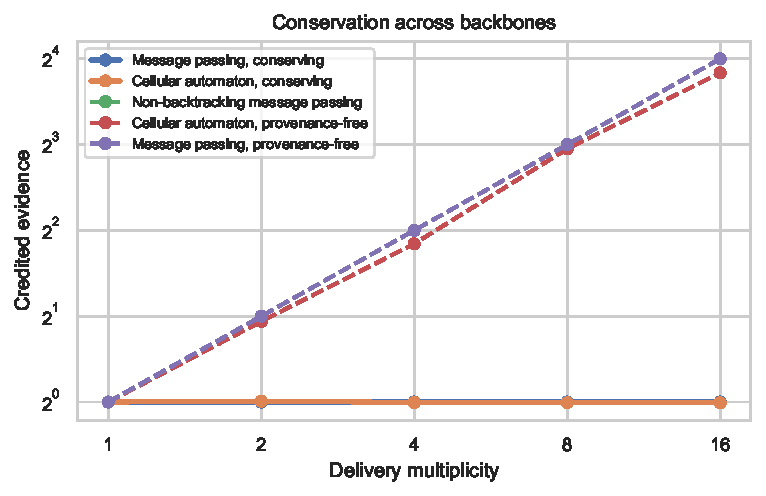
\includegraphics[width=0.66\textwidth]{figures/fig_conservation_backbones.pdf}
\caption{Credited evidence against delivery multiplicity on log-log axes, five
seeds. The horizontal rule marks exact conservation. Conserving arms stay on
that rule, while provenance-free arms and the non-backtracking baseline track
the identity.}
\label{fig:backbones}
\end{figure}

Duplication also degrades a matched provenance-free message-passing network by
$6.144$ nats more in negative log-likelihood than the conserving one.
Table~\ref{tab:cost} reports end-to-end time on a common workload. The ledger
suppresses arrivals before they reach the content path, which is why its total
falls below that of no defence. MinHash and embedding detection spend roughly
eight times as long as the ledger in their accounting stage.

\begin{table}[h]
\centering\small
\caption{End-to-end cost on a common workload of $4{,}674$ delivered messages.
Ledger time is the accounting overhead and content time is the learned path.}
\label{tab:cost}
\resizebox{\textwidth}{!}{%
\begin{tabular}{lccccc}
\toprule
Accounting rule & Delivered & Reaching content & Accounting (ms) & Content (s) & Total (s) \\
\midrule
\textbf{Lineage ledger (this work)} & $4{,}674$ & $984$ & $1.36$ & $0.030$ & $\mathbf{0.037}$ \\
Canonical hashing \citep{lee2022deduplicating} & $4{,}674$ & $984$ & $1.34$ & $0.031$ & $0.037$ \\
SimHash \citep{charikar2002simhash} & $4{,}674$ & $984$ & $1.42$ & $0.031$ & $0.038$ \\
MinHash \citep{broder1997resemblance} & $4{,}674$ & $984$ & $10.65$ & $0.031$ & $0.080$ \\
Embedding detection \citep{xiao2023bge} & $4{,}674$ & $984$ & $11.15$ & $0.030$ & $0.082$ \\
No defence & $4{,}674$ & $4{,}674$ & $0.07$ & $0.063$ & $0.063$ \\
\bottomrule
\end{tabular}}
\end{table}

The frozen-reader efficiency measurement of Section~\ref{sec:transfer} uses
Qwen2.5-1.5B-Instruct \citep{qwen2025qwen25} on the first $\ReaderRecords$
two-hop records.

\section{Semantic-Sybil audit}
\label{app:sybil}

The audit measures how far fabricated identities can inflate credited
evidence when each fabricated source carries a meaning-preserving paraphrase.

\paragraph{Generation and acceptance.} For each of $\SybPopulation$ AVeriTeC
claims, eight paraphrase candidates of the source are generated with
Qwen2.5-0.5B \citep{qwen2025qwen25} at a pinned revision under deterministic
decoding. The candidate corpus is frozen before any evaluation. A candidate is
accepted only if it entails and is entailed by the original under a pinned
natural language inference model, and only if its surface similarity to the
original is below $\SybSurfaceThreshold$. The first test excludes candidates
that changed the meaning, and the second excludes near-copies that surface
deduplication would already catch.

\paragraph{Semantic grouping.} The BGE \citep{xiao2023bge} cosine threshold of
$\SybThreshold$ is fitted on training pairs only, under a maximum false-link
budget of $0.5\%$ fixed in advance. On $\SybPositivePairs$ positive and
$\SybNegativePairs$ negative training pairs it attains recall $\SybRecall$ at a
realised false-link rate of $\SybFalseLinkPct\%$. Of $\SybPopulation$ claims,
$\SybEligible$ retain enough accepted paraphrases to support multiplicity
eight.

\begin{table}[h]
\centering\small
\caption{Credited evidence under the paraphrase attack, five seeds over
$\SybEligible$ eligible claims. Credit is relative to the single-source
baseline.}
\label{tab:sybil}
\begin{tabular}{lccccc}
\toprule
Grouping & Multiplicity & Credit ratio & $95\%$ interval & NLL & Flip rate \\
\midrule
% generated by analysis/final_paper_macros.py
URL identity & $1$ & $1.000$ & $[1.000, 1.000]$ & $1.1212$ & $0.0000$ \\
 & $2$ & $2.060$ & $[1.995, 2.126]$ & $1.1056$ & $0.0467$ \\
 & $4$ & $4.131$ & $[4.030, 4.233]$ & $1.1496$ & $0.0433$ \\
 & $8$ & $4.567$ & $[4.328, 4.807]$ & $1.1394$ & $0.0600$ \\
\addlinespace
canonical URL & $1$ & $1.000$ & $[1.000, 1.000]$ & $1.1212$ & $0.0000$ \\
 & $2$ & $2.060$ & $[1.995, 2.126]$ & $1.1056$ & $0.0467$ \\
 & $4$ & $4.131$ & $[4.030, 4.233]$ & $1.1496$ & $0.0433$ \\
 & $8$ & $4.567$ & $[4.328, 4.807]$ & $1.1394$ & $0.0600$ \\
\addlinespace
surface family & $1$ & $1.000$ & $[1.000, 1.000]$ & $1.1212$ & $0.0000$ \\
 & $2$ & $2.016$ & $[1.945, 2.088]$ & $1.1046$ & $0.0467$ \\
 & $4$ & $3.363$ & $[3.230, 3.497]$ & $1.1302$ & $0.0433$ \\
 & $8$ & $3.724$ & $[3.514, 3.933]$ & $1.1198$ & $0.0600$ \\
\addlinespace
semantic family & $1$ & $1.000$ & $[1.000, 1.000]$ & $1.1212$ & $0.0000$ \\
 & $2$ & $1.676$ & $[1.598, 1.754]$ & $1.0944$ & $0.0467$ \\
 & $4$ & $2.522$ & $[2.362, 2.682]$ & $1.1090$ & $0.0433$ \\
 & $8$ & $2.673$ & $[2.468, 2.878]$ & $1.0968$ & $0.0600$
\\
\bottomrule
\end{tabular}
\end{table}

Table~\ref{tab:sybil} shows that semantic grouping reduces the attack
substantially relative to identifier-based grouping, from $4.567$ to $2.673$ at
multiplicity eight, and that no grouping restores exact conservation. The
negative log-likelihood moves little across multiplicities, so fabricated
identities inflate credit more than they move the prediction.

\section{Reproducibility and compute}
\label{app:repro}

\paragraph{Models and revisions.} Passages for the learned models are encoded
with the $768$-dimensional BGE model \citep{xiao2023bge}, released as
\texttt{bge-base-en-v1.5}, at revision \texttt{a5beb1e3}. The frozen readers are
Qwen2.5-7B-Instruct and Qwen2.5-1.5B-Instruct \citep{qwen2025qwen25} in
bfloat16 with greedy decoding and $48$ new tokens, and the paraphrase generator
is Qwen2.5-0.5B. No encoder, reader or generator is fine-tuned anywhere in this
work.

\paragraph{Hardware.} The synthetic backbone matrix and the synthetic
directional models run on CPU. The learned MuSiQue memory, the Sybil audit and
the frozen readers run on an NVIDIA H100 80GB partition with PyTorch 2.5.1.

\paragraph{Seeds and scale.} The learned models use five seeds, $10{,}000$
iterations and a batch size of $128$, with roughly $0.5$M trainable parameters
over the frozen encoder. The frozen readers are deterministic, so their
uncertainty is estimated by resampling records.

\paragraph{Regeneration.} Each script below reads committed raw outputs and
writes the named artifacts.
% Long file paths cannot hyphenate, so the list is set ragged right.
\begin{itemize}\setlength{\itemsep}{0pt}\raggedright
\item \path{experiments/musique_syndication_eval.py}, run once per arrival
order, produces the frozen-reader syndication outputs.
\item \path{analysis/syndication_analysis.py} applies the pre-registered
decision rules and writes the verdict.
\item \path{analysis/story_tables.py} writes Tables~\ref{tab:syndication},
\ref{tab:prereg} and~\ref{tab:synd-full}, Figure~\ref{fig:syndication}, and
every syndication and reader number quoted in the text.
\item \path{experiments/musique_duplication_eval.py} and
\path{experiments/musique_reader_eval.py} produce the learned-memory and
reader-efficiency outputs, and \path{scripts/dgx_rechunk.sh} runs the
re-chunked and fragments sweeps.
\item \path{analysis/learned_memory_table.py} produces
Tables~\ref{tab:learned} and~\ref{tab:learned-full}.
\item \path{experiments/directional_synthetic.py},
\path{experiments/directional_musique.py} and
\path{analysis/directional_analysis.py} produce the directional results and
their verdict.
\item \path{analysis/axiom_predictions.py} and
\path{analysis/conservation_figures.py} produce Table~\ref{tab:taxonomy} and
Figure~\ref{fig:backbones}.
\end{itemize}

\end{document}
